%%%%%%%%%%%%%%%%%%%%%%%%%%%%%%%%%%%%%%%%%%%%%%%%%%%%%%%%%%%%%%%%%%%%%%%%%
%                                                                       %
% ustthesis_test.tex: A template file for usage with ustthesis.cls      %
%                                                                       %
%%%%%%%%%%%%%%%%%%%%%%%%%%%%%%%%%%%%%%%%%%%%%%%%%%%%%%%%%%%%%%%%%%%%%%%%%

\documentclass{ustthesis}

\usepackage{mathpazo,amsmath,amssymb,epsfig,enumerate,bbm,calc,color,ifthen,capt-of} % original was times, but I think it's ugly; we use the same as IEEE CompSoc
\usepackage{algorithm}
\usepackage[noend]{algorithmic}
\usepackage[center]{subfigure}
\usepackage{color,graphicx}
\DeclareGraphicsExtensions{.pdf,.png,.jpg,.jpeg} % for pdflatex we expect .pdf, .png, or .jpg files
\graphicspath{{figures/}{pictures/}{images/}{./}} % where to search for the images

\newtheorem{proof}{Proof}
\usepackage{hyperref} % for better viewing experience  -- added by alan
\renewcommand{\chapterautorefname}{Chapter}
\renewcommand{\sectionautorefname}{Section}
\renewcommand{\subsectionautorefname}{Section}
\renewcommand{\tableautorefname}{Table}

\usepackage[a4paper,total={170mm,257mm},left=20mm,top=20mm]{geometry}

%% it is recomended to use ``\autoref{sec:bla}'' instead of ``Fig.~\ref{sec:bla}''

% Alan: begin the font trial
% Euler for math | Palatino for rm | Helvetica for ss | Courier for tt
\renewcommand{\rmdefault}{ppl} % rm
%\linespread{1.05}        % Palatino needs more leading
\usepackage[scaled]{helvet} % ss
\usepackage{courier} % tt
%\usepackage{euler} % math
\usepackage{eulervm} % a better implementation of the euler package (not in gwTeX)
\normalfont
\usepackage[T1]{fontenc}
% Alan: end the font trial
\usepackage{multirow}

\newcommand{\red}[1]{#1}
\newcommand{\tab}[1]{\hspace{3mm}}

\newcommand{\etal}{\textit{et al}. }
\newcommand{\ie}{\textit{i}.\textit{e}.}
\newcommand{\eg}{\textit{e}.\textit{g}.}

% \usepackage{latexsym}
    % Use the "latexsym" package when encountering the following error:
    %   ! LaTeX Error: Command \??? not provided in base LaTeX2e.
% \usepackage{epsf}
    % Use the "epsf" package for including EPS files.

%%%%%%%%%%%%%%%%%%%%%%%%%%%%%%%%%%%%%%%%%%%%%%%%%%%%%%%%%%%%%%%%%%%%%%%%%
%                                                                       %
% Preambles. DO NOT ERASE THEM. Change to suite your particular purpose.%
%                                                                       %
%%%%%%%%%%%%%%%%%%%%%%%%%%%%%%%%%%%%%%%%%%%%%%%%%%%%%%%%%%%%%%%%%%%%%%%%%

\title{A Survey on Visualization for Explainable Classifiers}  % Title of the thesis.
\author{Yao~MING}     % Author of the thesis.
% \degree{\MPhil}             % Degree for which the thesis is.
%% or
%\degree{\PhD}              % Degree for which the thesis is.
\subject{Computer Science and Engineering}      % Subject of the Degree.
\department{Computer Science and Engineering}       % Department to which the thesis
                    % is submitted.
\advisor{Prof.~Huamin~Qu}     % Supervisor.
% \depthead{Prof.~Mounir~HAMDI}    % department head.
% \defencedate{2010}{06}{25}      % \defencedate{year}{month}{day}.

% NOTE:
%   According to the sample shown in the guidelines, page number is
%   placed below the bottom margin.  However, if the author prefers
%   the page number to be printed above the bottom margin, please
%   activate the following command.

% \PNumberAboveBottomMargin

\begin{document}

%%%%%%%%%%%%%%%%%%%%%%%%%%%%%%%%%%%%%%%%%%%%%%%%%%%%%%%%%%%%%%%%%%%%%%%%%
%                                                                       %
% Now the actual Thesis. The order of output MUST be followed:          %
%                                                                       %
%    1) TITLEPAGE                                                       %
%                                                                       %
% The \maketitle command generates the Title page as well as the        %
% Signature page.                                                       %
%                                                                       %
%%%%%%%%%%%%%%%%%%%%%%%%%%%%%%%%%%%%%%%%%%%%%%%%%%%%%%%%%%%%%%%%%%%%%%%%%

\maketitle

%%%%%%%%%%%%%%%%%%%%%%%%%%%%%%%%%%%%%%%%%%%%%%%%%%%%%%%%%%%%%%%%%%%%%%%%%
%                                                                       %
%     2) DEDICATION (Optional)                                          %
%                                                                       %
% The \dedication and \enddedication commands are optional. If          %
% specified it generates a page for dedication.                         %
%
%%%%%%%%%%%%%%%%%%%%%%%%%%%%%%%%%%%%%%%%%%%%%%%%%%%%%%%%%%%%%%%%%%%%%%%%%

% \dedication
% This is an optional section.
% \enddedication

%%%%%%%%%%%%%%%%%%%%%%%%%%%%%%%%%%%%%%%%%%%%%%%%%%%%%%%%%%%%%%%%%%%%%%%%%
%                                                                       %
%     3) ACKNOWLEDGMENTS                                                %
%                                                                       %
% \acknowledgments and \endacknowledgments defines the                  %
% Acknowledgments of the author of the Thesis.                          %
%                                                                       %
%%%%%%%%%%%%%%%%%%%%%%%%%%%%%%%%%%%%%%%%%%%%%%%%%%%%%%%%%%%%%%%%%%%%%%%%%

% \input{chapter/sec-ack}
%%%%%%%%%%%%%%%%%%%%%%%%%%%%%%%%%%%%%%%%%%%%%%%%%%%%%%%%%%%%%%%%%%%%%%%%%
%                                                                       %
%     4) TABLE OF CONTENTS                                              %
%                                                                       %
%%%%%%%%%%%%%%%%%%%%%%%%%%%%%%%%%%%%%%%%%%%%%%%%%%%%%%%%%%%%%%%%%%%%%%%%%

\tableofcontents

%%%%%%%%%%%%%%%%%%%%%%%%%%%%%%%%%%%%%%%%%%%%%%%%%%%%%%%%%%%%%%%%%%%%%%%%%
%                                                                       %
%     5) LIST OF FIGURES (If Any)                                       %
%                                                                       %
%%%%%%%%%%%%%%%%%%%%%%%%%%%%%%%%%%%%%%%%%%%%%%%%%%%%%%%%%%%%%%%%%%%%%%%%%

% \listoffigures

%%%%%%%%%%%%%%%%%%%%%%%%%%%%%%%%%%%%%%%%%%%%%%%%%%%%%%%%%%%%%%%%%%%%%%%%%
%                                                                       %
%     6) LIST OF TABLES (If Any)
%                                                                       %
%%%%%%%%%%%%%%%%%%%%%%%%%%%%%%%%%%%%%%%%%%%%%%%%%%%%%%%%%%%%%%%%%%%%%%%%%

% \listoftables

%%%%%%%%%%%%%%%%%%%%%%%%%%%%%%%%%%%%%%%%%%%%%%%%%%%%%%%%%%%%%%%%%%%%%%%%%
%                                                                       %
%     7) ABSTRACT                                                       %
%                                                                       %
% \abstract and \endabstract are used to define a short Abstract for    %
% the Thesis.                                                           %
%                                                                       %
%%%%%%%%%%%%%%%%%%%%%%%%%%%%%%%%%%%%%%%%%%%%%%%%%%%%%%%%%%%%%%%%%%%%%%%%%

% \makeabstract
\begin{abstract}

Classification is a fundamental problem in machine learning, data mining and computer vision. In practice, interpretability is a desired property of classification models (classifiers) in critical areas like security, medicine and finance. For instance, a quantitative trader may prefer a more interpretable model with less expected return due to its predictability. Unfortunately, most best-performing classifiers in many applications (e.g., deep neural networks) are complex machines whose predictions are difficult to explain. Thus, there is a growing interest in using visualization to understand, diagnose and explain machine learning systems in both academia and industry. Many challenges need to be addressed in the formalization of explainability and design principles and evaluation of explainable intelligent systems.

The survey starts with an introduction on the concept and background of explainable classifiers. Existing work in both visualization and machine learning communities is categorized in terms of data types and purposes of explanation. Then the survey ends with a discussion on the challenges and future research opportunities of explainable classifiers.

\end{abstract}


%%%%%%%%%%%%%%%%%%%%%%%%%%%%%%%%%%%%%%%%%%%%%%%%%%%%%%%%%%%%%%%%%%%%%%%%%
%                                                                       %
%     8) The Actual Contents                                            %
%                                                                       %
% The command \chapters MUST BE USED to ensure that the entire content  %
% of the Thesis is double-spaced (in version 1.0).                      %
%                                                                       %
% However, in version 2.0, \chapters will be automatically added in     %
% the beginning of the first chapter.                                   %
%                                                                       %
%%%%%%%%%%%%%%%%%%%%%%%%%%%%%%%%%%%%%%%%%%%%%%%%%%%%%%%%%%%%%%%%%%%%%%%%%

%%\chapters         % Not necessary with ustthesis.cls (v2.0).

%%%%%%%%%%%%%%%%%%%%%%%%%%%%%%%%%%%%%%%%%%%%%%%%%%%%%%%%%%%%%%%%%%%%%%%%%
%                                                                       %
% Each chapter is defined via the \chapter command. The usual sectional %
% commands of LaTeX are also available.                                 %
%                                                                       %
%%%%%%%%%%%%%%%%%%%%%%%%%%%%%%%%%%%%%%%%%%%%%%%%%%%%%%%%%%%%%%%%%%%%%%%%%


\chapter{Introduction}\label{sec-introduction}

Placeholder for introduction.

\newpage

\chapter{Concepts and Definitions}\label{sec-concepts}

In this section, we first briefly introduce the problem of classification, as an instance of supervised learning, and a few popular classifications models (classifiers). To clarify the scope of this survey, we discuss the concepts of explainability of classifiers and illustrate in which circumstances explainability are desirable or needed. 

% \section{Concepts and Definitions}

% To clarify the scope of this survey, we first briefly introduce the problem of classification, as an instance of supervised learning, and a few popular classifications models (classifiers). 

%% Briefly Introduce classification

\section{Classification} \label{sec:classifier-classification}

Given an input space $\mathcal{X}$ and an output space $\mathcal{Y}=\{1, 2, ..., K\}$ with $K$ classes, \textbf{classification} is the problem of identifying any \textbf{observation} $\mathbf{x}\in\mathcal{X}$ to a class $y\in\mathcal{Y}$. For multi-label classification, where class labels are not exclusive, we can view it as multiple related binary classification. For simplicity, we only consider the basic formulation in this survey. 

A \textbf{classifier} is an algorithm $f$ that implements classification, \ie, $y = f(\mathbf{x})$. To handle ambiguity, a classifier is often used in a probabilistic setting. That is, the output of $f$ a probabilistic distribution $p(y\mid \mathbf{x}, \mathcal{D})$ over all possible classes in $\mathcal{Y}$. $\mathcal{D}$ is the training set, which is a subset of $\mathcal{X}\times\mathcal{Y}$, that have already been observed. Thus, in practice, a classifier will often take the form of $\mathbf{y} = f(\mathbf{x})$, where $\mathbf{y}=(y_i)\in\mathbb{R}^K$ is a vector denoting the probabilistic distribution. Then the final classification will be the class $i$ with largest probability $\arg\max_{i}{y_i}$.

% The \textbf{learning} or training of a classifier is the process of determining the best $f\in\mathbf{F}$ based on a given training set $\mathbf{D}$ that minimizes our cost of error, or, \textbf{loss function}. 

\section{Classifiers}

Classification is now widely applied in solving many real world applications. A few examples are: face recognition [], handwritten recognition [], sentiment analysis [] and spam filtering. 
Here we briefly present a few popular models for classifications, including $k$-nearest neighbors, support vector machines, decision trees and neural networks.

\textbf{$K$-nearest neighbor}.

\textbf{Support vector machine}.

\textbf{Decision trees}.

\textbf{Neural networks}. CNN, RNN.

\section{Explainability}

What is explainability? What is the explainability of a classifier? There is no commonly agreed definitions so far. Doshi-Velez and Kim defines interpretability (or explainability) as the ability to explain or to present in understandable terms to a human \cite{doshi-velez2017interpretableml}, which is already a good general definition. To clarify the scope of this survey, we define the \textbf{explainability} of a classifier as the ability to explain the reasoning of its predictions so that a human can understand. Simple models such as a linear classifier already has good explainability since humans can easily understand the model's reasoning by simply looking at the coefficients of each feature. For a complicated classifier like a deep neural network, a human may find it difficult to understand due to layer-wise structure and the nonlinearity of the computation. Thus, the key of explainability is the humans.

An immediate question is: why do we need explainability? 
%Aren't existing complex and high-performing classifiers good enough? 
The need of explainability for a full automated classifier mainly comes from three aspects: humans' curiosity about knowledge, limitations of current intelligent algorithms, and moral and legal issues:

\begin{itemize}
  \item \textbf{Curiosity of human}. Humans are curious about new knowledge. % in the data, and the knowledge learned by the model. 
  Often, a classifier is not developed solely for performing the classification tasks, but also for knowledge discovery. For todays popular neural networks, humans are curious of how the impressive human-level classification accuracy is achieved. There are also examples of how insights learned from the behavior of a model lead to improvement on the design of a classifier \cite{zeiler2014eccv, alsallakh2017cnn-hierarchy}. Besides, given that AlphaGo Zero \cite{silver2017mastering} can learn to master the game of Go much better than human players, it is desirable that the machine can explain its learned strategy (knowledge) to us.
  \item \textbf{Limitations of machines}. The current state-of-the-art intelligent systems are usually not fully testable. Human knowledge are required as a complement in case the machines fail. In the seeable future, machines are expected to assist rather than replace humans in many domains, such as security, medical services, education and design. By providing explainability, users' trust can be more easily established. Besides, explainability can provide an interface for humans to monitor machine.
  \item \textbf{Moral and legal issues}. The ``right to explanation'', which is a regulation included in the GDPR \footnote{\url{https://www.privacy-regulation.eu/en/r71.htm}} of the European Union, has recently raised a debate on to which extent we should require automatic decision-making systems to provide explanations to the subjects of the decision. If one's application for a loan is denied by a automatic classifier, he/she has the right to ask why. A doctor may need to know why a patient is classified to have a lung cancer to give the final diagnosis. Another issue is the fairness or the discrimination problem of a classifier, which may be easily neglected during the development phase.
\end{itemize}

Though explainability is a desirable property, it should be noted that it is not always necessary. Explainability is not required if 1) the application domain has high resistance to errors, and thus, unexpected errors is acceptable; 2) the application domain has been well studied and the classifier has been well tested in production, and thus, it is unlikely to have unexpected results.

\newpage
\chapter{Explainable Classifiers}\label{sec-explainable-classifier}

In this section, we discuss methods that provide explainability to classifiers. We categorized related work into two depending on how the explainability of a classifier is achieved. 
%namely, interpretable classifiers that are recognized to be easy to understand, generating explanations for classifiers that are difficult to understand.

% \section{Concepts and Definitions}

% % To clarify the scope of this survey, we first briefly introduce the problem of classification, as an instance of supervised learning, and a few popular classifications models (classifiers). 

% %% Briefly Introduce classification

% \subsection{Classification} \label{sec:classifier-classification}

% Given an input space $\mathcal{X}$ and an output space $\mathcal{Y}=\{1, 2, ..., K\}$ with $K$ classes, \textbf{classification} is the problem of identifying any \textbf{observation} $\mathbf{x}\in\mathcal{X}$ to a class $y\in\mathcal{Y}$. For multi-label classification, where class labels are not exclusive, we can view it as multiple related binary classification. For simplicity, we only consider the basic formulation in this survey. 

% A \textbf{classifier} is an algorithm $f$ that implements classification, \ie, $y = f(\mathbf{x})$. To handle ambiguity, a classifier is often used in a probabilistic setting. That is, the output of $f$ a probabilistic distribution $p(y\mid \mathbf{x}, \mathcal{D})$ over all possible classes in $\mathcal{Y}$. $\mathcal{D}$ is the training set, which is a subset of $\mathcal{X}\times\mathcal{Y}$, that have already been observed. Thus, in practice, a classifier will often take the form of $\mathbf{y} = f(\mathbf{x})$, where $\mathbf{y}=(y_i)\in\mathbb{R}^K$ is a vector denoting the probabilistic distribution. Then the final classification will be the class $i$ with largest probability $\arg\max_{i}{y_i}$.

% % The \textbf{learning} or training of a classifier is the process of determining the best $f\in\mathbf{F}$ based on a given training set $\mathbf{D}$ that minimizes our cost of error, or, \textbf{loss function}. 

% \subsection{Classifiers}

% Classification is now widely applied in solving many real world applications. A few examples are: face recognition [], handwritten recognition [], sentiment analysis [] and spam filtering. 
% Here we briefly present a few popular models for classifications, including $k$-nearest neighbors, support vector machines, decision trees and neural networks.

% \textbf{$K$-nearest neighbor}.

% \textbf{Support vector machine}.

% \textbf{Decision trees}.

% \textbf{Neural networks}. CNN, RNN.

% \subsection{Explainability}

% What is explainability? What is the explainability of a classifier? There is no commonly agreed definitions so far. Doshi-Velez and Kim defines interpretability (or explainability) as the ability to explain or to present in understandable terms to a human \cite{doshi-velez2017interpretableml}, which is already a good general definition. To clarify the scope of this survey, we define the \textbf{explainability} of a classifier as the ability to explain the reasoning of its predictions so that a human can understand. Simple models such as a linear classifier already has good explainability since humans can easily understand the model's reasoning by simply looking at the coefficients of each feature. For a complicated classifier like a deep neural network, a human may find it difficult to understand due to layer-wise structure and the nonlinearity of the computation. Thus, the key of explainability is the humans.

% An immediate question is: why do we need explainability? 
% %Aren't existing complex and high-performing classifiers good enough? 
% The need of explainability for a full automated classifier mainly comes from three aspects: humans' curiosity about knowledge, limitations of current intelligent algorithms, and moral and legal issues:

% \begin{itemize}
%   \item \textbf{Curiosity of human}. Humans are curious about new knowledge. % in the data, and the knowledge learned by the model. 
%   Often, a classifier is not developed solely for performing the classification tasks, but also for knowledge discovery. For todays popular neural networks, humans are curious of how the impressive human-level classification accuracy is achieved. There are also examples of how insights learned from the behavior of a model lead to improvement on the design of a classifier \cite{zeiler2014eccv, alsallakh2017cnn-hierarchy}. Besides, given that AlphaGo Zero \cite{silver2017mastering} can learn to master the game of Go much better than human players, it is desirable that the machine can explain its learned strategy (knowledge) to us.
%   \item \textbf{Limitations of machines}. The current state-of-the-art intelligent systems are usually not fully testable. Human knowledge are required as a complement in case the machines fail. In the seeable future, machines are expected to assist rather than replace humans in many domains, such as security, medical services, education and design. By providing explainability, users' trust can be more easily established. Besides, explainability can provide an interface for humans to monitor machine.
%   \item \textbf{Moral and legal issues}. The ``right to explanation'', which is a regulation included in the GDPR \footnote{\url{https://www.privacy-regulation.eu/en/r71.htm}} of the European Union, has recently raised a debate on to which extent we should require automatic decision-making systems to provide explanations to the subjects of the decision. If one's application for a loan is denied by a automatic classifier, he/she has the right to ask why. A doctor may need to know why a patient is classified to have a lung cancer to give the final diagnosis. Another issue is the fairness or the discrimination problem of a classifier, which may be easily neglected during the development phase.
% \end{itemize}

% Though explainability is a desirable property, it is not always necessary. Explainability is not required if 1) the application domain has high resistance to errors, and thus, unexpected errors is acceptable; 2) the application domain has been well studied and the classifier has been well tested in production, and thus, it is unlikely to have unexpected results.

%To achieve explainability, existing work mainly falls into two categories. 
The first type of work develops more interpretable classifiers that are easy to understand for humans. The second generates explanations for a classifier without modifying the model, either by explaining the classifier locally on specific instances, or by explaining the behavior of the classifier globally. A summary is shown in \autoref{tab:explainable-methods}.

\renewcommand{\arraystretch}{1.3}

\begin{table}[hb]
  \centering
\begin{tabular}{ |c|c|c|p{15em}|p{7.5em}| } 
  \hline
  \multicolumn{3}{|c|}{Categories} & Related Papers & Remarks \\
  \hline
  \multirow{10}{6em}{\centering Interpretable Classifiers} & \multicolumn{2}{|c|}{\multirow{5}{6em}{\centering Interpretable Architecture}}
  & Decision Trees \cite{breiman1984classificationtree}, & \multirow{3}*{rule-based} \\
  & \multicolumn{2}{|c|}{} & Rule Lists \cite{letham2015stroke, wang2015falling}, & \\ 
  & \multicolumn{2}{|c|}{} & Rule Sets \cite{wang2017rulesets} & \\ 
  \cline{4-5}
  & \multicolumn{2}{|c|}{} & Linear Models \cite{debock2010gam} & linear \\ 
  \cline{4-5}
  & \multicolumn{2}{|c|}{} & kNNs \cite{dudani1976weightedknn,keller1985fuzzyknn} & instance-based \\ 
  \cline{2-5}
  & \multicolumn{2}{|c|}{\multirow{5}{6em}{\centering Learning Sparse Models}}
  & Decision Trees \cite{quinlan1987simplifying}, & \multirow{3}*{simplification} \\
  & \multicolumn{2}{|c|}{} & Sparse SVMs \cite{downs2001simplifysvm}, & \\
  & \multicolumn{2}{|c|}{} & Sparse CNNs \cite{liu2015sparsecnn} & \\
  \cline{4-5}
  & \multicolumn{2}{|c|}{} & Sparsity by Bayesian \cite{tipping2001sparse}, & \multirow{2}*{direct-sparsity} \\
  & \multicolumn{2}{|c|}{} & Integer Models \cite{tan2010sparsesvm,ustun2016supersparse} & \\
  \hline
  \multirow{14}{6em}{\centering Explanations of Classifiers} & \multirow{9}{3em}{\centering Local} & \multirow{3}{4em}{\centering Model-unaware}
  & Sensitivity Analysis \cite{simonyan14saliency,li2016naccl-hlt,smilkov2017smoothgrad} & gradient-based \\ 
  \cline{4-5}
  & & & LIME \cite{ribeiro2016kdd} & model induction \\ 
  \cline{4-5}
  & & & Generate Visual Explanations \cite{hendricks16generate} & extra labels \\ 
  \cline{3-5}
  & & \multirow{5}{4em}{\centering Model-aware}
  & De-convolution \cite{zeiler2014eccv}, & CNN \\
  & & & Layer-wise Propagation \cite{bach15plos}, & CNN \\
  & & & Prediction Difference \cite{zintgraf17visualize}, & Image \\
  & & & Output Decomposition \cite{murdoch2017rule}, & LSTM \\
  & & & Direct Mapping \cite{karpathy16rnn} & RNN \\
  \cline{2-5}
  & \multirow{4}{3em}{\centering Global} & \multirow{1}{4em}{\centering Unaware}
  & LIME \cite{ribeiro2016kdd} & model induction  \\ 
  \cline{3-5}
  & & \multirow{3}{4em}{\centering Model-aware}
  & Partition Hidden Space \cite{feraud2002nn,rauber2017hidden-activity}, & NN \\
  & & & Activation maximization \cite{erhan2009techreport}, & CNN \\
  & & & Network Dissection \cite{bau2017netdissect} & CNN \\
  \hline
\end{tabular}
\caption{Towards explainable classifiers.}
\label{tab:explainable-methods}
\end{table}

\section{Interpretable Classifiers}\label{sec:interpretable-classifier}

\textbf{Interpretable classifiers} are the classifiers that are commonly recognized to be more understandable than others, and hence, do not need extra explicit explanations. Summarizing existing work, we find two major strategies for creating interpretable classifiers: developing interpretable models with easy-to-understand structures, and learning simpler or sparser models.

\subsection{Interpretable Architecture}

To create more interpretable classifiers, a natural way is to use simple computation structures (\eg, if-then rules). Most classifiers that fall into this category are rule-based. 

\textbf{Rule-based}. A widely adopted type of models are the decision trees \cite{breiman1984classificationtree}. A decision tree classifier uses internal nodes and branches to represent its classification reasoning as conjunctions of rules. A human can trace back a specific classification from a leaf to the root to understand the prediction of the classifier. However, the difficulty of constructing a high-accuracy and interpretable decision tree has long been criticized. 

Focused on balancing among performance, explainability and computation, a few recent studies introduce the Bayesian framework in rule-based classifiers. Letham \etal \cite{letham2015stroke} develop the Bayesian Rule List (BRL) which employs a prior structure that encourages sparsity in the generated decision lists with a good accuracy. The rule lists have the form of if-then-else structures, as shown in \autoref{fig:bayesian-rule-list}. Wang and Rudin \cite{wang2015falling} design the Falling Rule Lists that use an ordered if-then rule list so that the most at-risk occasion will be handled first. Wang \etal \cite{wang2017rulesets} construct rule sets based on AND and OR operations and highlight its low computation cost and on-par accuracy compared with SVM and random forest.

% \footnotetext{{https://umbrella.cisco.com/blog/2013/06/13/server-side-software-and-malware-analysis/} }

\begin{figure}[tb]
  \centering
  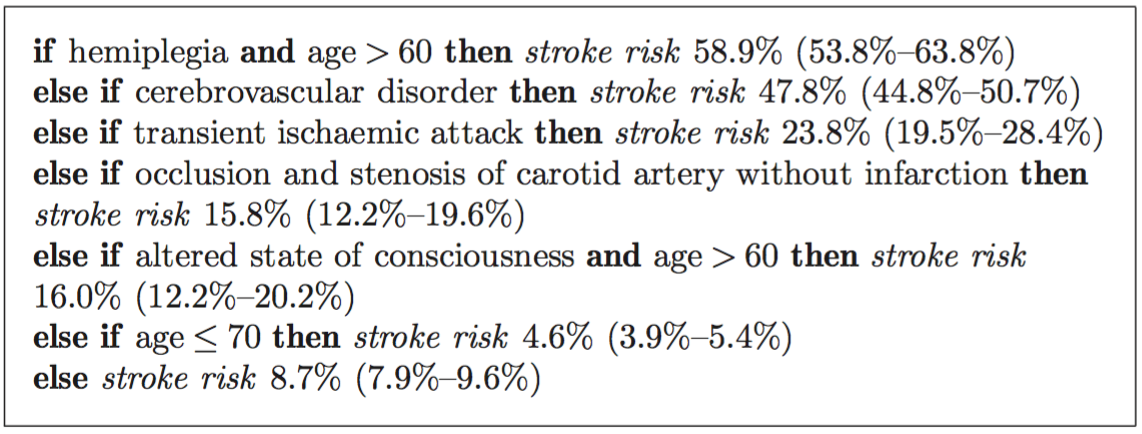
\includegraphics[width=0.9\textwidth]{figure/bayesian-rule-list}
  \caption{A decision list learned by the BRL algorithm \cite{letham2015stroke}.}
  \label{fig:bayesian-rule-list}
\end{figure}

\begin{figure}[tb]
  \centering
  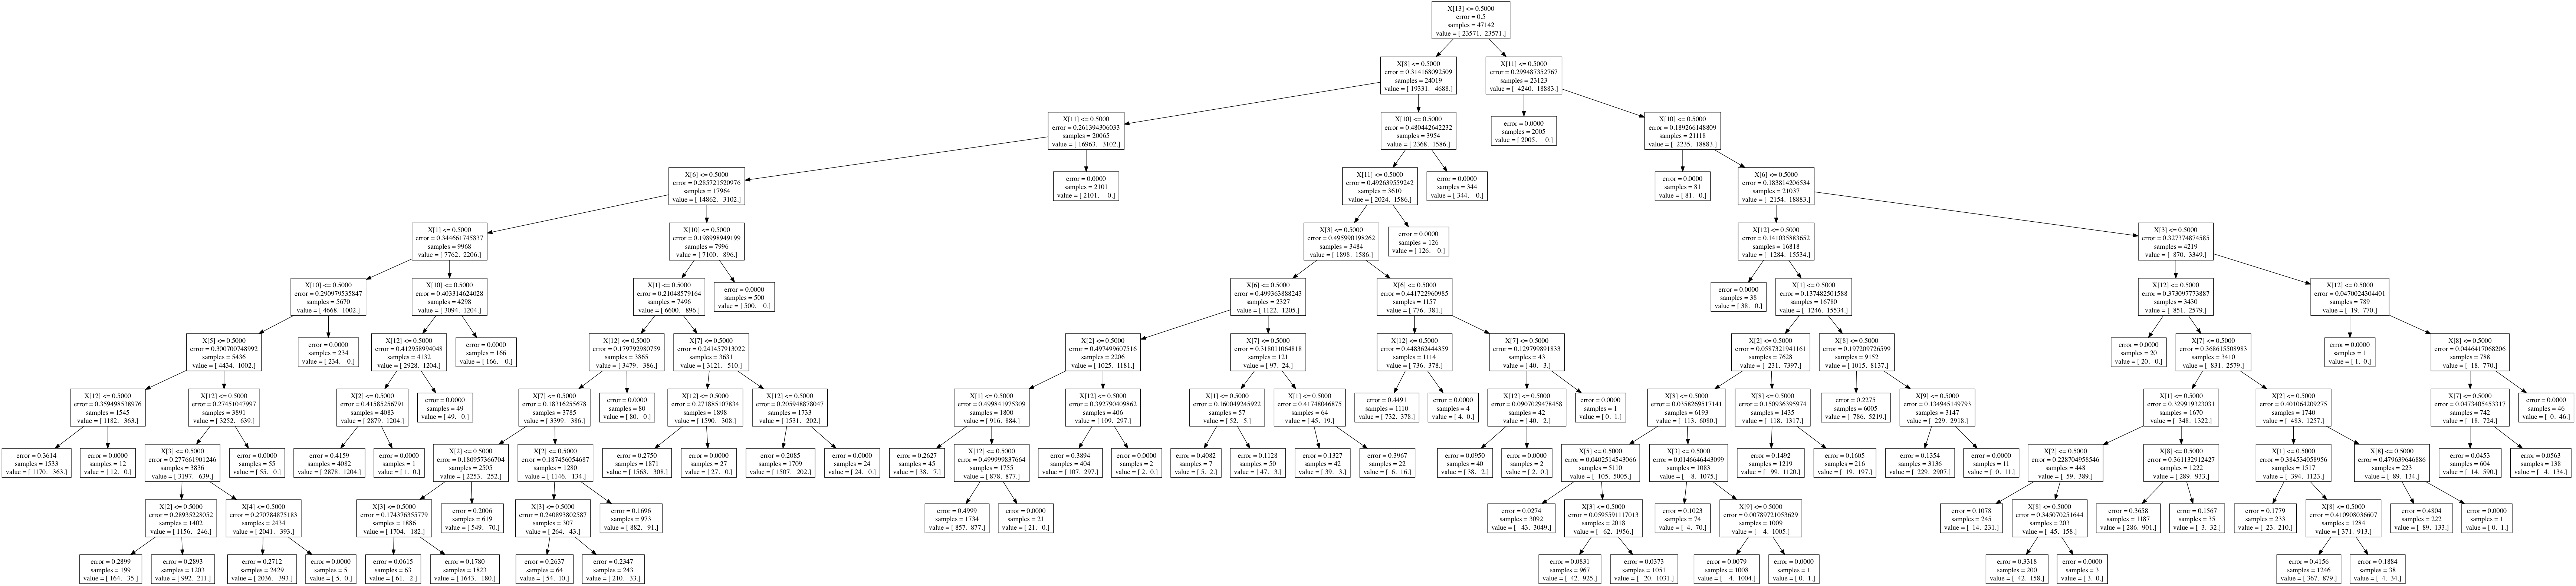
\includegraphics[width=1.0\textwidth]{figure/huge-tree}
  \caption{A decision tree with over one hundred nodes, which is hard to explain its reasoning.}
  \label{fig:huge-tree}
\end{figure}

The most series problem of these interpretable models with easy-to-understand structures is the scalability. The performance of the rule-based models increases as the number of rules increases or the non-linearity increases. Although the rule-based models are easy to learn and understand at the first glance, it is intractable to understand the classifier as a whole when the number of nodes of rules grows up to a few hundreds. An example is shown in \autoref{fig:huge-tree}.

\textbf{Others}. Except for rule-based models, there are a few other models with more complicated models are recognized to be interpretable.
One family of interpretable models worth noticing are the generalized linear models \cite{debock2010gam}, which are pervasive in statistics and finance. Although these models can have highly nonlinear computations, the additive relation between nonlinear functions of features are believed to be easy-to-understand. However, the generalized linear classifiers can also be hard to understand when their non-linearity increased to a certain extent. The other non-probabilistic family of classifiers are the $k$-nearest neighbors (kNN) classifiers, whose prediction can be easily understood by presenting the observation's $k$-nearest neighbors. Numerous work has been done to boost the performance the kNN classifiers, including weighted kNN with different kernels \cite{dudani1976weightedknn} and fuzzy kNN \cite{keller1985fuzzyknn}. The explainability of kNN classifiers may easily fail when there lacks good neighbors for certain observations.

% \subsection{Learning Interpretable Representations}

% Instead of restricting the classifier to the combination of simple computations, some other work dedicates to learn more interpretable representations from the data. For example, Maier \etal [] learning causal knowledge from relational representations

% Features used by the model are easily interpretable.

% e.g. KNN


% Translation \cite{bahdanau2014translation}.
% Image Captioning \cite{xu15icml}.

\subsection{Learning Sparse Models}

As discussed above, the explainability often decreases as the complexity (\ie, number of parameters or nodes) of the model increases. Thus, we can improve the explainability by learning a sparser model with the same architecture. Two common strategies are used to learn a sparse model: simplifying a ``dense'' model through pruning or approximation; introducing sparsity as a prior to learn a sparse model from scratch. 
% These methods can also be regarded as model compressions, which reduce computation costs. 

% Note that learning sparse neural networks are not part of this category, since they focus on reducing the computation cost rather than explainability.

\textbf{Simplification}. The methods for simplifying classifiers are usually developed in a model-specific manner. Quinlan summarizes four techniques for simplifying decision trees \cite{quinlan1987simplifying}, \ie, cost-complexity pruning, reduced error pruning, pessimistic pruning and simplification to rule sets. Downs \etal \cite{downs2001simplifysvm} recognize and eliminate dependent support vectors while leaving the outputs of SVM unchanged. Liu \etal \cite{liu2015sparsecnn} use a sparse decomposition method to zero out redundant parameters in a CNN, achieving about 10-times speedup while only losing about 1\% accuracy. Though these methods can practically simplify classifiers and speed up computations, they do not directly provide explainability. A simplified SVM with fewer support vectors but utilizing a complicated kernel is still difficult to explain. A simplified decision tree with 200 nodes instead of 1,000 nodes is still hard to interpret.

\textbf{Learning from scratch}. To directly learn sparser models from scratch, Tipping \cite{tipping2001sparse} proposed a general Bayesian framework that treats sparsity as a prior and specialized this method on SVM. Instead of restricting the complexity of the parameters, Tan \etal \cite{tan2010sparsesvm} uses a 0-1 control variable to each input feature, and convert the learning to a mixed integer programming problem. Similar idea can be found in the sparse linear integer models proposed by Ustun \etal \cite{ustun2016supersparse}. Although these methods can learn sparse classifiers without losing much performance, they mainly focus on reducing the computation costs instead of providing explainability. They do not guarantee explainability if the classification problem is difficult.

In most cases, the efforts of developing more interpretable classifiers are tradeoffs between performance and explainability. For performance-critical applications, it is always difficult to train a interpretable classifier that do not need extra explanations.

% A common problem of these interpretable classifiers, either by using simple structures or by learning sparser models, is that their explainability depends on the data itself. If the inputs $\mathbf{x}$ are intrinsically difficult to explain,

\section{Explanations of Classifiers}

Generating explanations of a classifier without modifying the classifier itself is preferred when the underlying model is already too complicated, \eg, neural networks and SVMs, and we don't want to sacrifice performance. There is also no common-recognized definition for what an \textbf{explanation} of a classifier is. Most existing work uses a subset or a weighted subset of input features to explain a single prediction of a classifier, \eg, a mask over the input image, a heatmap with the same size as the input image, a bag of words or categorical fields. Some work \cite{ribeiro2016kdd} proposed to induct a simpler classifier (\eg, linear classifier) as the explanation of a prediction. Here we only discuss explanations for complex classifiers. Thus, illustrative diagrams for simple classifiers are not included here.

In cognitive science, explanations are characterized as arguments that demonstrating all or a subset of the causes of the \textbf{explanandum} (the subject being explained), usually following deductions from natural laws or empirical conditions \cite{hempel1948explanation,lombrozo2006explanation}. Here we give a general definition: 

\textbf{Explanations of a classifier} is the human-understandable representations that identify the causes of the classifier's prediction(s). A typical form of human-understandable representations is the visualization. As introduced in \autoref{sec:classifier-classification}, a classifier can be regarded as a function $f$, which is in general learned from a training dataset $\mathcal{D}$, specified by learned parameters $\theta$. Thus, the \textbf{causes} can traced to 1) parts of the training data $\mathcal{D}$, 2) parts of the parameters $\theta$ as some components of the classifier, or 3) parts of the input, $x$, of a prediction or predictions. 

If an explanation is provided to explain $f$'s prediction in a small region around a given input point $\mathbf{x}$, we call it as a \textbf{local explanation}. If it is generated to explain $f$ on the whole input space $\mathcal{X}$ in general or as a summary, we call it as a \textbf{global explanation}. Sometime, we also want to have an intermediate \textbf{subset explanation} that is performed on a subset $\mathcal{S}$ of $\mathcal{X}$, in which the inputs share some common features. 
%The global explanation can actually be regarded as a extreme case of subset explanation, where $\mathcal{S}=\mathcal{X}$. 
Next, we discuss the related work on explanations of classifiers based on the above taxonomy. 

%They are viewed as the central to our sense of understanding and the currency in which we exchange concepts \cite{lombrozo2006explanation}.

% \subsection{Definitions of Explanation}

% A review of how previous work define explanations in machine learning.

% General: ML:\cite{doshi-velez2017interpretableml}. Cognitive:\cite{lombrozo2006explanation}

% Data-type specific definitions: image-based, text-based, categorical data.

% Some other work focuses on explaining the model itself (the mechanism, compositions of the model) to facilitate the understanding and diagnosing of the model.

% To summarize, no agreed definition of explanation of classifier exists. Here we give a general definition...Next we give problem specific definitions.

% Learned from surveying the literature, we separate the problem of explaining classifiers into two sub-tasks: explaining the predictions of classifiers (instance-level); explaining the classifier itself (model-level).

% For each sub-tasks, the existing methods can be divided into two types: model-aware explanations and model-unaware explanations.


\subsection{Local Explanations}

As we have discussed, the causes used in an explanation of a classifier can be the training data, model parameters, and inputs. For local explanation, the input $\mathbf{x}$ is always specified and used in the explanation. Depending on whether an explanation is generated directly using model's parameters or structures, we categorize local explanation methods into model-aware and model-unaware methods.

\begin{figure}[tb]
  \centering
  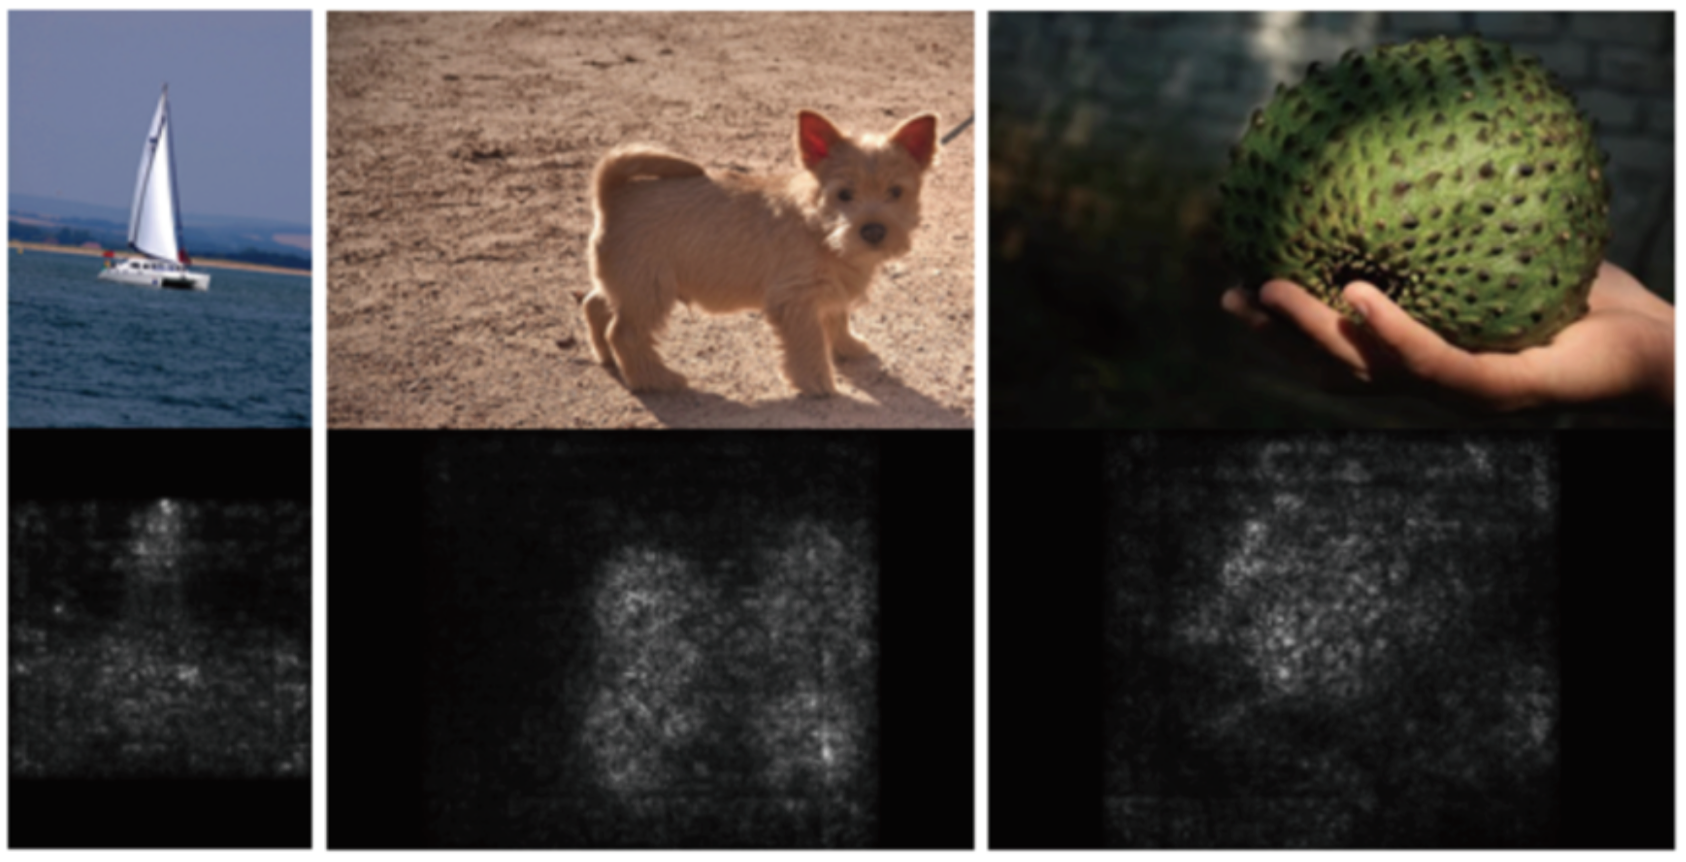
\includegraphics[width=1.0\textwidth]{figure/saliency-map}
  \caption{Images (first row) and their saliency maps (second row) for the top-1 predicted class in ILSVRC-2013 test images \cite{simonyan14saliency}.}
  \label{fig:saliency-map}
\end{figure}

\begin{figure}[tb]
  \centering
  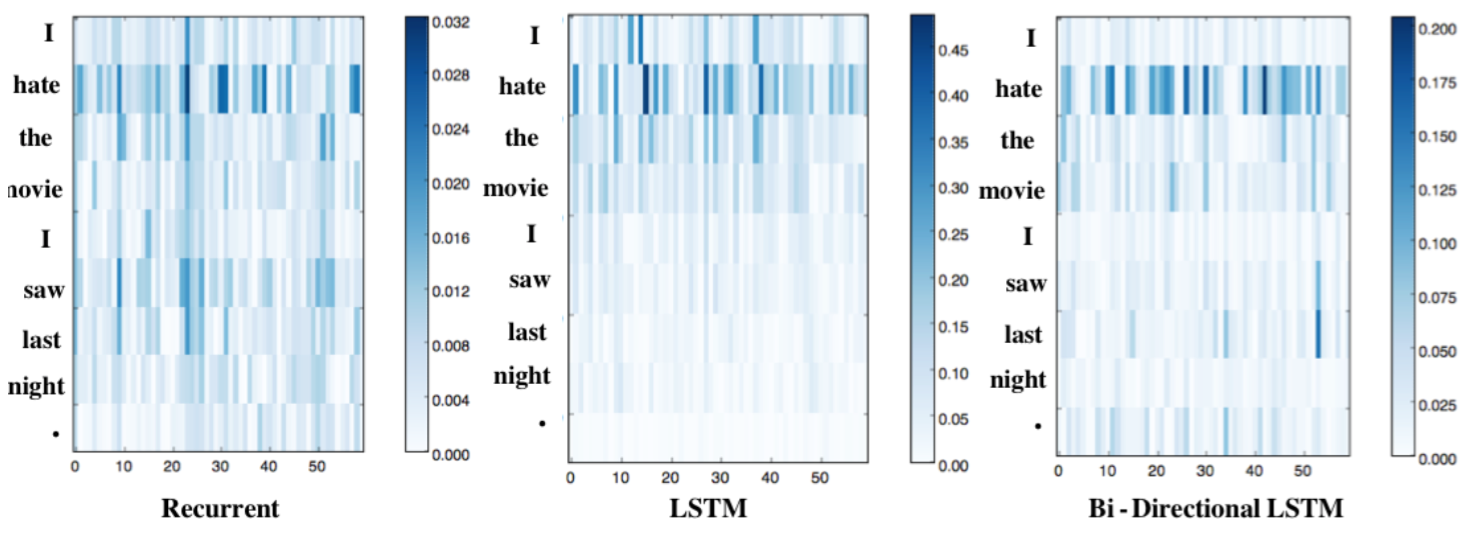
\includegraphics[width=1.0\textwidth]{figure/saliency-map-rnn}
  \caption{Saliency matrix maps for ``I hate the movie I saw last night.'' of three RNN sentiment classifiers. \textit{Left}: a vanilla RNN; \textit{Middle}: an LSTM; \textit{Right}: a bi-directional LSTM \cite{simonyan14saliency}.}
  \label{fig:saliency-map-rnn}
\end{figure}

\textbf{Model-unaware explanations} only require the input $\mathbf{x}$ and a computable $f$. Most work uses sensitivity or saliency-based techniques to derive explanations. Simonyan \etal \cite{simonyan14saliency} use the derivative of a image classifier $f_i$ w.r.t. the input image $\mathbf{x}$ as the saliency score of the class $i$, and map the score of each pixel to a saliency map as the explanation of $\mathbf{x}$. Li \etal \cite{li2016naccl-hlt} also calculate the derivative of a text sentiment RNN classifier w.r.t. the embeddings of an input sentence (which is a matrix), as shown in \autoref{fig:saliency-map-rnn}. The heatmap matrices are used as explanations for users to identify salient dimensions of the embedding vector and salient words that contribute the most to the prediction. Although these sensitivity-based methods are intuitive and can be efficiently approximated, their generated explanations are often noisy (as shown in \autoref{fig:saliency-map}), due to the high nonlinearity of the complicated classifier. Recently, Smilkov \etal \cite{smilkov2017smoothgrad} propose a random sampling technique to smooth the gradient, which achieve more meaningful visual explanations. However, this smoothing technique is computationally expensive and non-deterministic.

Instead of sensitivity analysis, some other work trains another model to explain the explanandum. Ribeiro \etal \cite{ribeiro2016kdd} approximate a complicated classifier locally using a simple linear classifier, and proceed to generate super-pixel patches as explanations. This method is actually similar to the gradient smoothing, since the training of the linear classifier is also done by sampling around the current input. Forming the problem as image captioning, Hendricks \etal \cite{hendricks16generate} use extra labeled explanation texts of images to train a explainer that generate explanatory texts of a image classifier. This method highly depends on the quality of text explanations labels, which require extra expensive labeling. Besides, it introduces another model, which is another potential explanandum that need to explain.

% image data: \cite{simonyan14saliency,zeiler2014eccv,bach15plos,zintgraf17visualize}

% text data: \cite{karpathy16rnn,li2016naccl-hlt,martens2014explaindocument,arras2017rnn-sentiment}

\begin{figure}[tb]
  \centering
  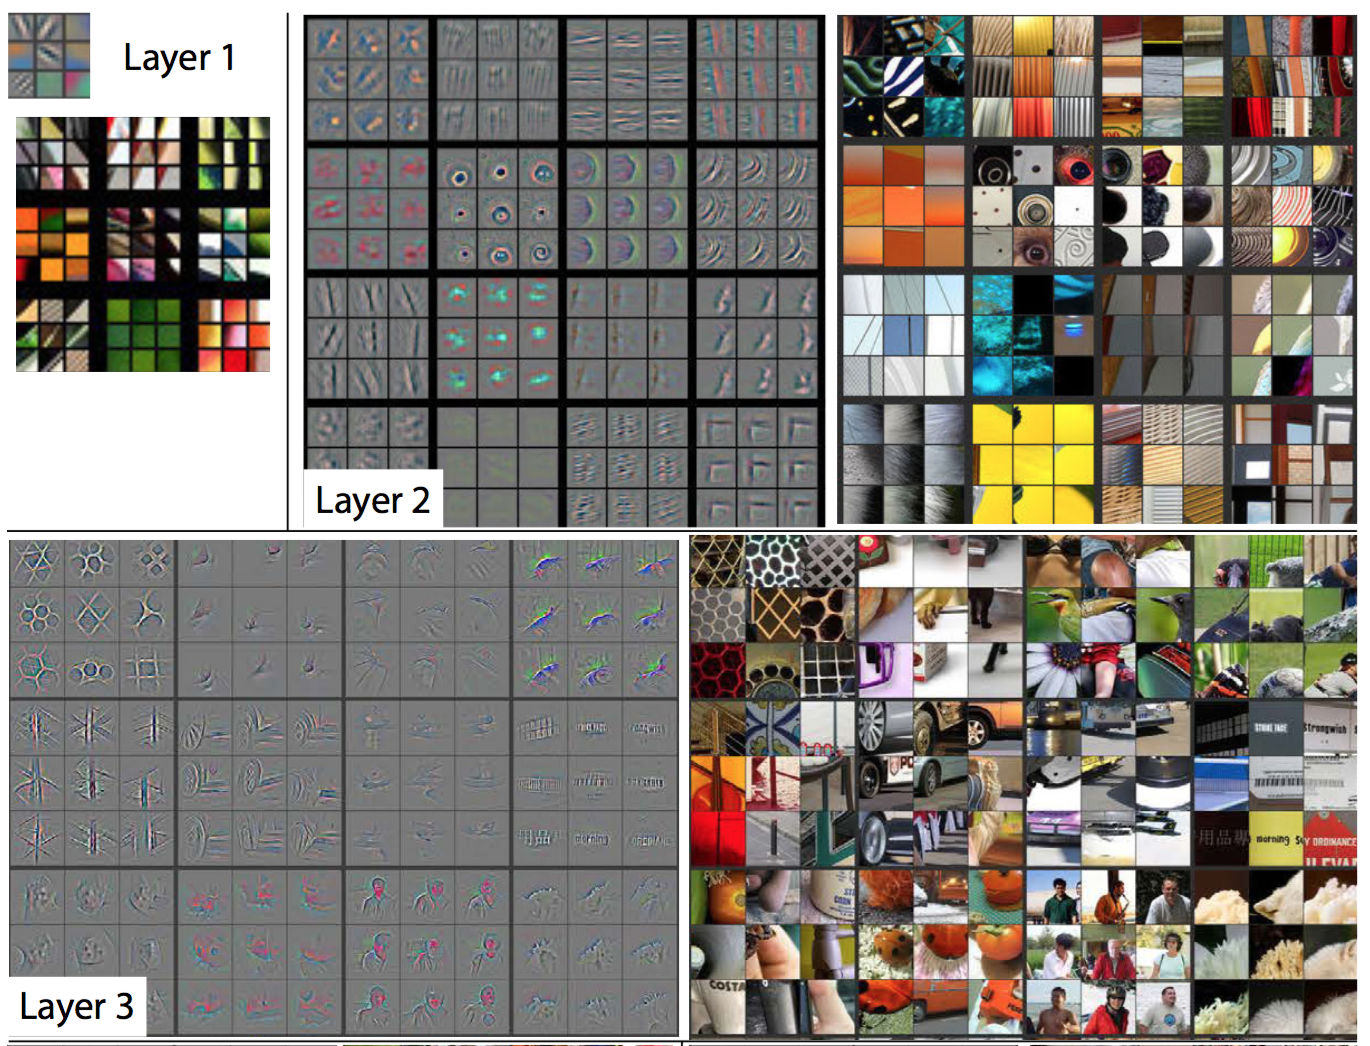
\includegraphics[width=1.0\textwidth]{figure/deconv}
  \caption{Visualization of a CNN generated using the de-convolution method \cite{zeiler2014eccv}. Gray images in the left are the top nine activations in a random subset of neurons across validation data, projected back to image space. In the right are corresponding image patches.}
  \label{fig:deconv}
\end{figure}

\textbf{Model-aware explanations} utilize another cause -- the parameters of the model, $\theta$, to amplify the information in the explanation. Zeiler and Fergus \cite{zeiler2014eccv} developed a de-convolution method that map the outputs of a CNN classifier back to the input space, utilizing the inverse operations of different layers. The projected images \autoref{fig:deconv} can be used as an explanation of what different neurons are usede for. Bach \etal \cite{bach15plos} uses a layer-wise relevance propagation (LRP) that improves the sparsity of the image heatmap. Zintgraf \etal \cite{zintgraf17visualize} developed a visualization that highlight evidence for and against a prediction seperately through prediction difference analysis. Murdoch and Szlam \cite{murdoch2017rule} decomposed the output of an LSTM classifier into multiplicative contribution scores of input words and uses the scores to explain how important the words are for the prediction. Though these methods typically result in much better (sparse, meaningful) explanations than model-unaware methods, they are developed in a per-model manner, which are hard to generalize for other classifiers. There is a lack of general explanatory frameworks to guide and evaluate the development of model-aware methods. Flooded by the interest in deep learning, we can hardly find methods developed for classification models other than neural networks.

% Erhan \etal \cite{erhan2009techreport} developed the activation maximization method that generate 

Using the cause of training data for explanations has not attracted interest until recently. Koh and Liang proposed a fast approximation of the influence function, which is a well-studied method in statistics. The influence functions can help identifying training points that are most responsible for a given prediction \cite{koh2017influencefunctions}, and thus can explain the prediction from the aspect of training data.
 
\subsection{Global Explanations}
The global explanations are not dependent on any specific inputs. A global explanation is actually a summary of the reasoning of how a classifier generally behaves. Unlike local explanations which are defined around a certain point, the global explanations are considered to be ill-posed and are much harder to achieve. Similarly to local explanations, we divide existing work into model-aware and model-unaware methods.

\textbf{Model-unaware explanations}. To our knowledge, very few methods has been proposed to generate global explanations for general classifiers. Ribeiro \etal \cite{ribeiro2016kdd} proposed to select a collection of representative local explanations and present to the users one local explanation at a time to give a global understanding. This method will easily fail when the dataset (training data) is too large. The users will not be able to remember a lot representative local explanations to form a global understanding.

% \cite{ribeiro2016kdd} Image and text, sampling instanc-level explanations

\textbf{Model-aware explanations}. The first attempt to understand a complex classifier globally is done by F{\'e}raud and Cl{\'e}rot \cite{feraud2002nn}. They partitioned the hidden representation space through clustering the representation of the whole training set, where each cluster represent a semantic concept learned by the classifier. To qualitatively understand a CNN, Erhan \etal \cite{erhan2009techreport} proposed the activation maximization method. Each neuron in the CNN can be explained using an image patch that will maximize its activation. 
% Ming \etal \cite{ming2017vast} summarize the functions of different hidden units of an RNN classifier using collections of words through co-clustering and find interesting semantic clusters in the hidden state. 
To provide conceptual meanings of the explanation, Bau \etal \cite{bau2017netdissect} align hidden units with human understandable concepts (objects) through a dissection process. However, these methods often require explorations over multiple nodes or neurons. The big picture is often neglected. Additionally, a common issue is that it is hard to compare these methods due to the lack of an evaluation framework.

% RNN: \cite{ming2017vast}

% CNN: \cite{bau2017netdissect} study interpretable units

% NN: \cite{feraud2002nn}

% \section{Research Issues}

In summary, there are two common strategies to make a classifier explainable. First, we develop simpler or sparser classifiers that can meet the performance requirements. Second, we build another human-understandable interface for explanation on top of a classifier. Both strategies are useful in different scenarios. 

However, an important, but neglected aspect of existing methods is the human. Few have paid attention to model human. Most of them study the classifiers and develop techniques for explainability and then argue that their methods help humans to understand the classifier, without studying how humans exactly response to the results generated by these techniques. 

Another related problem raised by Doshi-velez and Kim \cite{doshi-velez2017interpretableml} is the lack of the evaluation methods for explainability. Without a rigorous evaluation, it is hard to compare which method is better in a certain setting. It will also be infeasible to clarify the gap of current research and direction for future research.
% Address the problem of evaluation, and how other work evaluates.

\newpage
\chapter{Visualization for Explainable Classifiers}\label{sec-visualization}

As discussed at the end of \autoref{sec-explainable-classifier}, current research only focuses on one subject of the problem of explainable classifier and neglects the other subject -- human. Thus, we study explainable classifier from the aspects of visualization and human computer interaction in this chapter. Broadly speaking, the visualization for explainable classifiers can be viewed as a special case of algorithm visualization or software visualization. The former aims to provide better understanding of algorithms for education purposes in computer science. The latter focus on assisting developers and operation engineers for the development and maintenance of complex software. Here, the subject of visualization is the classifiers, which can be treated as algorithms learned from the data, or complex systems that need assistance in understanding.
% Unlike the previous chapter that discuss various algorithms for enhancing the explainability of classifiers,

We view the development and the operation of an intelligent system as a system engineering problem, and divide the life cycle of an intelligent system into different stages. The classification system can be treat as a specification of the general intelligent system. Then, we identify the current issues in explaining classifiers and discuss the research opportunities of visualization regarding different stages.

\section{Life Cycle of an intelligent system}

\begin{figure}[hb]
    \centering
    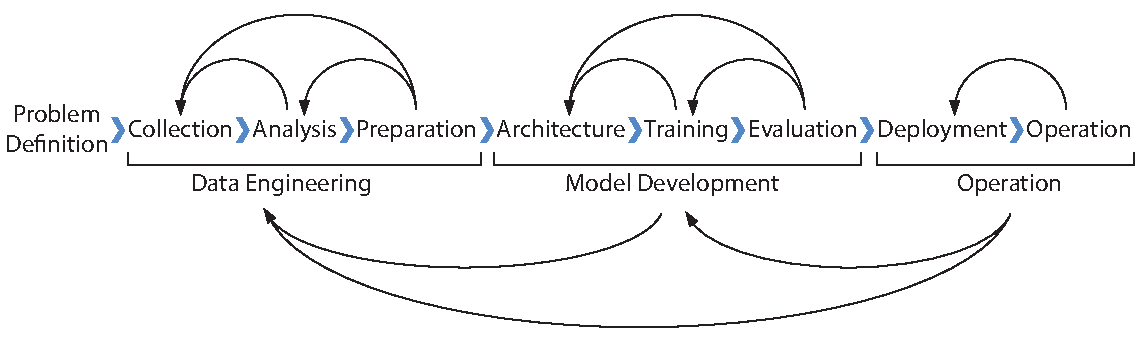
\includegraphics[width=1.0\textwidth]{figure/life-cycle}
    \caption{The life cycle of a classifier.}
    \label{fig:life-cycle}
\end{figure}

A classification system can be thought as a specialized case af an intelligence system. An intelligent system is developed to perform certain tasks with artificial intelligence (here we only consider data-driven systems). 
The development of a data-driven intelligent system is an iterative process. In this survey, the entire life cycle of an intelligent system is divided into three major stages (data engineering, model development, and operation) and eight sub-procedures (see \autoref{fig:life-cycle}). This definition is formed based on the cross-industry standard process for data mining \cite{wirth2000crisp}, a professional advice from Gartner, Inc. \cite{carlton2017ml}, the life cycle for expert system \cite{lasalle1990expert-system}, and the machine learning workflow of Google Cloud\footnote{\url{https://cloud.google.com/ml-engine/docs/ml-solutions-overview}}.

The first stage, data engineering, is defined to include any procedures that are data-related, namely, data collection, exploratory analysis, data preparation. The second stage, model development, includes procedures such as designing the architecture of the classifier (\eg, what type of model to use and parameters), training the model using data prepared, and evaluating whether the model meets certain requirements. After developing a classifier, the model is deployed, and in certain cases, is operated by some people. As we can see from \autoref{fig:life-cycle}, there are back-links from each stage/step to its previous stages/steps. This is the nature development. For example, we have a model with unsatisfactory performance after the training. This might due to model used is not suitable for certain tasks (go back to architecture setting), or it is because the volume of the data is too small (go back to collect more data). Similar problems might occur in other stages or procedures, which force us to go back and improve. 
%For example, if we are to develop a system for hospitals to detect early signs of lung cancer from a CT scan, the procedure goes as: 

Visualization and visual analytics systems are semi-automatic solutions at different stages to make a classifier more explainable. In the stage of data engineering, data visualization can help humans explore the data and get a qualitative sense of the nature of the data. Since the training of a classifier is actually extracting information from the training data, with more knowledge of the data in mind, humans (\ie developers or data scientists) can better understand if a failure results from the quality or volume issues of the data. At the second stage, visual analytics systems serve as development tools, which make the development more transparent and understandable. When designing or selecting model architectures, visual analytics systems can help humans better understand the characteristics of different classifiers, and even inspire improvements in the architecture. Visual diagnosing tools can help identify the problems in the training process and improve the debugging efficiency. For evaluations, visual analytics systems can help compare different classifiers and qualitatively evaluate the robustness and fairness of a classifier. At the last stage, when a classification system is deployed, visualization can help explain the inner workings of the system to end-users. For routine operations, visualization can better explain the predictions of the system, which make the monitoring and management easier. Also note that, visualization can used in the life-cycle for other purposes instead of explainability. For example, monitoring the training process by plotting loss curves, or visualization for crowd sourcing to collect data with better quality.

% -------

% A table summarizing all related papers

% -------

\section{Visualization for Data Understanding}

In the stage of data engineering, visualization can be used mainly in the procedure of data analysis to assist humans' understanding of the data. Data plays an important role in the success of machine learning advances. A trained classifier can be viewed as a machine that has extracted the information in the training data and abstracted the information as its parameters. Different classifiers are suitable for datasets with different characteristics. Besides, a classifiers performance is largely depend on the quality of its training data. Thus, understand the data is the first step to understand a classifier.

There is a long history of research in visualization for exploratory data analysis. When comes to the classification problem, the data involved is \textbf{multi-dimensional data} with categorical labels, usually having the type of images, texts and categorical data. There are mainly three tasks for understanding the data: statistical analysis, dimensionality reduction, and dataset diagnostics.

\begin{figure}[hbt]
    \centering
    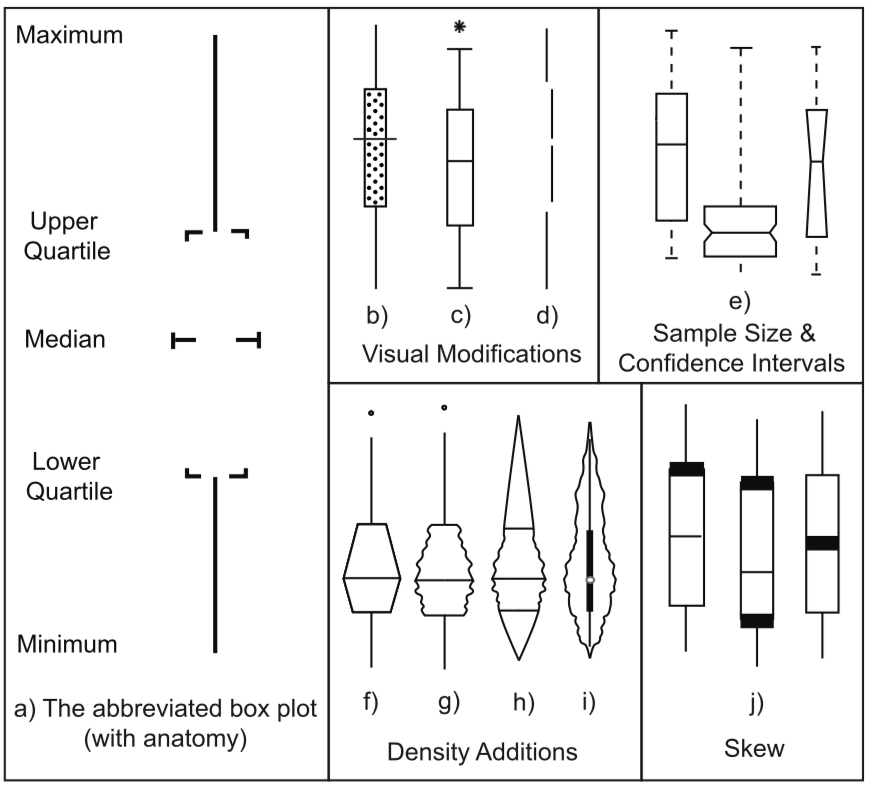
\includegraphics[width=0.7\textwidth]{figure/box-plots}
    \caption{Variations on the box plot \cite{potter2010statistics}. a) Abbreviated box plot. b) Range plot. c) Box plot. d) Interquartile plot. e) Variable width and notched box plots expressing sample sizes and confidence levels. f) Hist plot. g) Vase plot. h) Box-percentile plot. i) Violin plot. j) Skew and modality plots.}
    \label{fig:box-plots}
\end{figure}

\textbf{Statistical analysis}. The purpose of statistical analysis is to summarize statistical features of the datasets and provide users with a statistical understanding. One of the most influential visualization design is the box plot, which summarizes the key statistics of each feature in a box-like visualization. A survey on the design of box plots is provided by Potter \etal \cite{potter2010statistics}. As shown \autoref{fig:box-plots}, (a) presents the key features of a box plot. The box plots can be enhanced to embed more information such as confidence intervals in (e) and distribution densities in (f-i), providing more comprehensive summaries than the simple box plot. However, the datasets used in classification systems have become increasingly complex, with very high dimensions. Navigating through hundreds of box plots not necessarily provide insights about the datasets.

\begin{figure}[hbt]
    \centering
    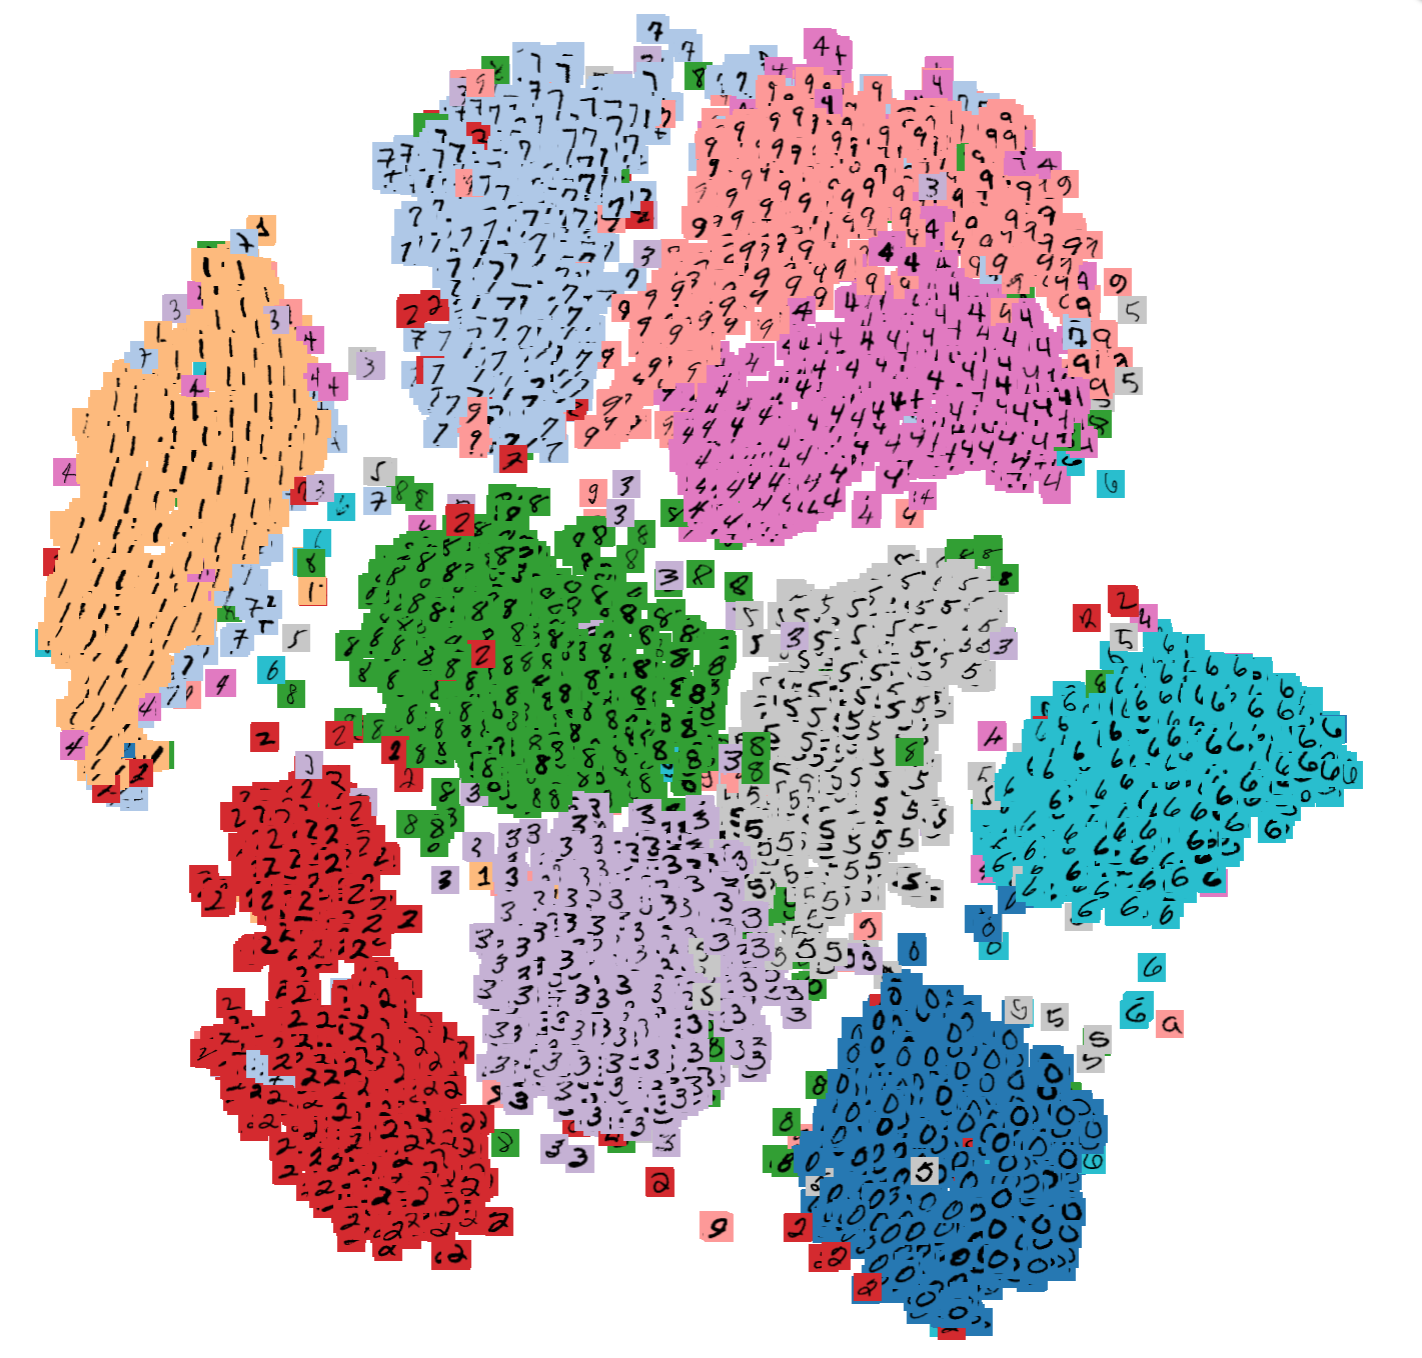
\includegraphics[width=0.7\textwidth]{figure/projector}
    \caption{The t-SNE projection of the MNIST dataset, colored by the labeled digits.}
    \label{fig:projector}
\end{figure}

\textbf{Dimensionality reduction}. In exploratory analysis, dimensionality reduction is usually applied for understanding how the data is distributed in the input space. Thus, projection, including principle component analysis (PCA), multidimensional scaling (MDS) \cite{kruskal1978mds}, and t-distributed stochastic neighbor embedding (t-SNE) \cite{maaten2008tsne}, is the most common dimensionality reduction technique used in this stage. The role of visualization is to present and augment the results of dimensionality reduction. A most recent example is the Embedding Projector \cite{smilkov2016projector}, which embed human interpretable labels (\eg, images with categorical colors ) in the scatter plots achieved by dimensionality reductions. By navigating the projected plot, users can better understand the relationship of different instances and identify clusters and outliers. For example, as shown in \autoref{fig:projector}, we can see that digits ``3'', ``5'' and ``8'' are actually very close to each other, and the classifier might have difficulties to distinguish them.

\textbf{Dataset diagnostics}. Diagnostics is an important and comprehensive task for improving the quality of the dataset. Given that different datasets usually have different characteristics, there is few automatic methods that can solve all the problems. Thus, human is required to be in the loop. The visualization techniques involved may vary for different datasets. Most commonly used are scatter plots, stacked diagrams, and their variations. An example visual dataset diagnostics tool for machine learning is the Facets\footnote{\url{https://github.com/PAIR-code/facets}}.

As discussed above, visualization techniques can help users develop understandings of the distribution, characteristics, and possible challenges of the datasets. These insights can guide the implementation and evaluation in the second stage of model development. In this sense, it is easier for developers to understand the behavior of classifiers, which makes the classification system more explainable. 

There are two research issues for visualization in the stage of data engineering. The first is the scalability issue. The volume of datasets can be very large (\eg, millions of instances), which brings about challenges in real-time visualization rendering and interaction designs. The second is the lack of comprehensive visual analytics system that are designed specifically for the development of intelligent systems. A developer will have to switch among different tools to perform different tasks, which need a lot of redundant work for format transformations. 
% There are a few examples such as WEKA\cite{hall2009weka}. 

% \textbf{Cluster analysis}. Projection, 

\section{Visualization for Model Development}

There is a surge of interest to use visualization in the stage of model development for explainable classifiers. We summarized three tasks for visualization, namely, model understanding, model diagnosing, and assessment and comparison, which are corresponding to the three stages: architecture design, training, and evaluation.

\begin{figure}[hbt]
    \centering
    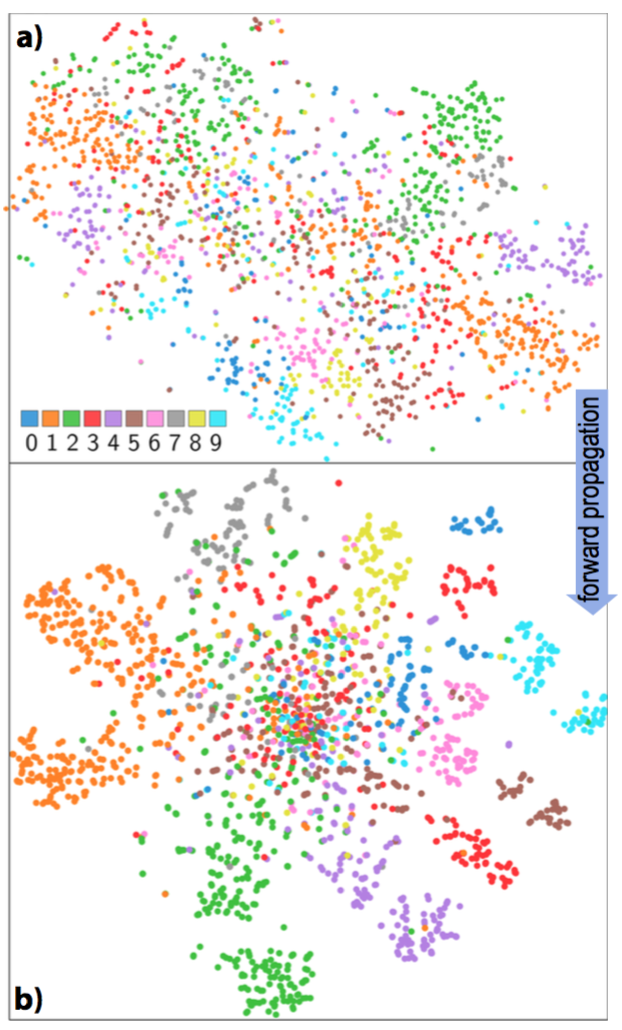
\includegraphics[width=0.5\textwidth]{figure/project-nn}
    \caption{Projection of the MLP hidden layer activations after training \cite{rauber2017hidden-activity}, SVHN test subset. a) First hidden layer. b) Last hidden layer.}
    \label{fig:project-nn}
\end{figure}

\subsection{Understanding}
The purposes of this task is to help researchers and developers better understand the characteristics and working mechanisms of different classifiers so that they can design a better one or choose a better one. The selection and design of the architecture of a classifier always require a strong expertise in machine learning, which needs cumulative experience of trial and error. For classifiers whose characteristics are still under studying (\eg, neural networks), such knowledge is even harder to achieve. Thus, most of the related work using visualization techniques for understanding classifiers focuses of neural networks. Considering the taxonomy of explanations, these visualizations mostly fall into model-aware global explanations, which provide a general sense of how a classifier behaves globally. Unlike pure explanation generation techniques, the visual analytics systems often embed extra information of the classifiers that boost understanding.
% Scientific understanding. Investigate the characteristic of the model.
These techniques can be roughly categorized into two: representation-based and component-based.

\textbf{Representation-based} methods visualize how a given set of instances is represented in the hidden layer or the final output of the classifier. As shown in \autoref{fig:project-nn}, Rauber \etal \cite{rauber2017hidden-activity} project the representations of a subset of instances in different layer, and verified that each layer of the network transform its input space to a more separable one. Unlike component-based methods, representation-based methods actually treat a model or a layer as a black box, and visualize how the representation space is transformed. This technique has been integrated in visual diagnostics systems such as ActiVis \cite{kahng2017activis} and DeepEyes \cite{pezzotti2017deep-eyes}. However, they are unable to analyze the detail information embedded in the classifiers.

\begin{figure}
    \centering
    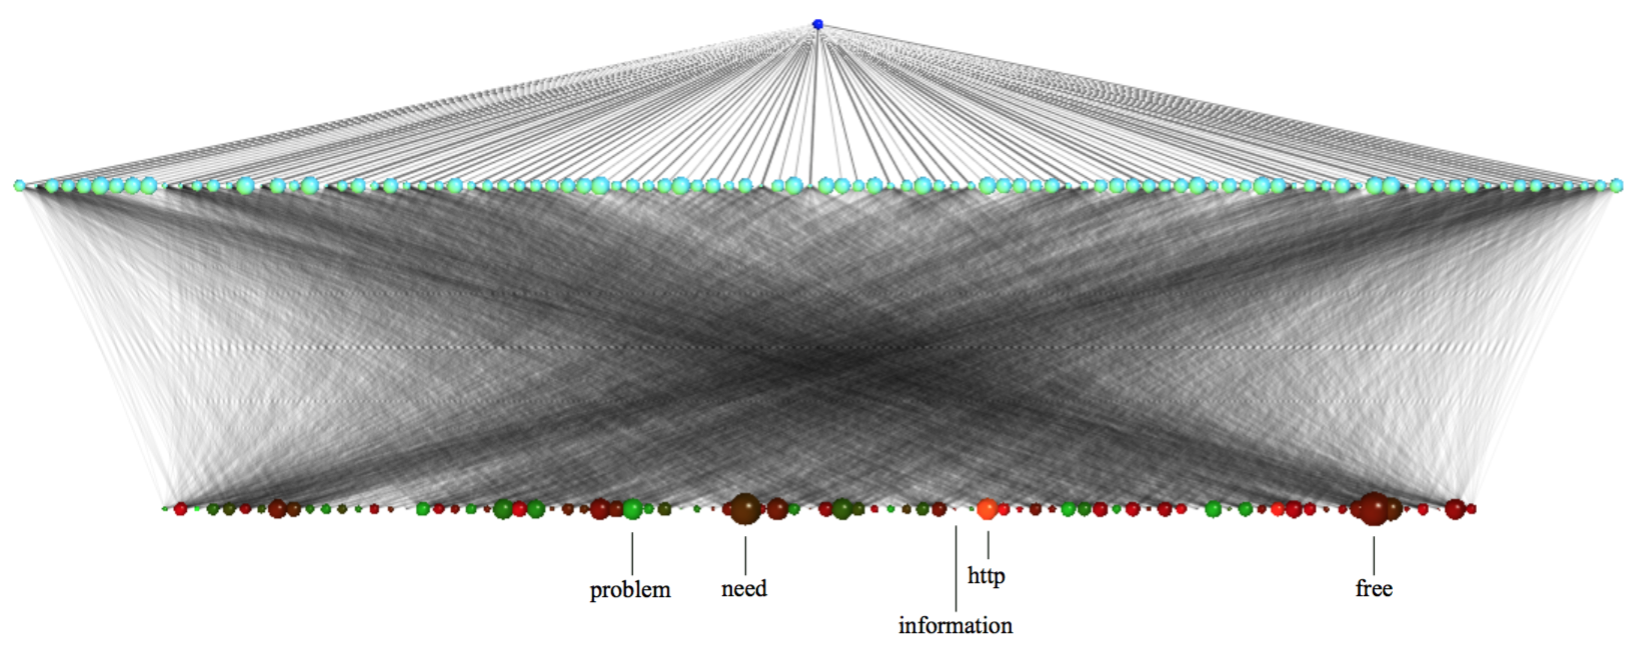
\includegraphics[width=1.0\textwidth]{figure/tzeng-nn}
    \caption{A spam classifier, where each input is a term in the email. The input data of the network is a subset of the spam in the training set \cite{tzeng2005visualize-nn}.}
    \label{fig:tzeng-nn}
\end{figure}

\begin{figure}
    \centering
    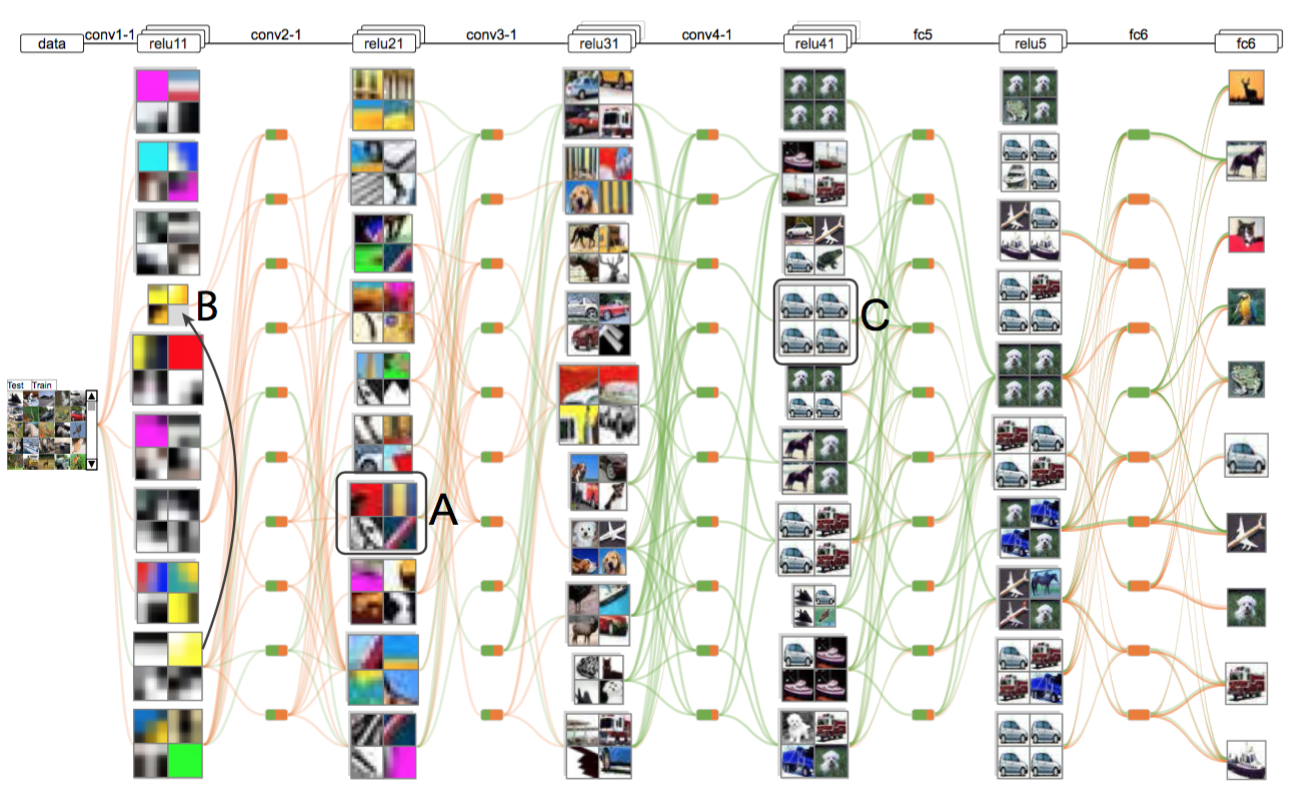
\includegraphics[width=1.0\textwidth]{figure/cnnvis}
    \caption{A visualization of a CNN with a large number of layers and neurons using neuron clustering and edge aggregation \cite{liu2017cnnvis}.}
    \label{fig:cnnvis}
\end{figure}

\textbf{Component-based} methods visualize the working mechanisms of specific components of a classifier. Tzeng and Ma directly visualize a multi-layer perceptron as a graph using the node-link layout. As shown in \autoref{fig:tzeng-nn}, though this visualization explained how important different term are for the neural network, it is visually cluttered and cannot reveal how neurons are combined to perform the classification. To provide more scalable visualization, Liu \etal develop the CNNVis \cite{liu2017cnnvis}, which use clustering and edge aggregation to provide a more compact visualization for CNNs. The representative image patch that activating each neuron clusters are also embedded in the visualization (see \autoref{fig:cnnvis}). There is also some work using visualization to understand RNNs. Karpathy \etal \cite{karpathy16rnn} visualize the value of a hidden unit along a sequence as a heatmap and find some hidden units have clear semantics. Strobelt \etal \cite{strobelt2017lstmvis} develop the LSTMVis based on parallel coordinates to identify dynamic patterns in the hidden state of an RNN. Ming \etal \cite{ming2017vast} develop the RNNVis, which is based on co-clustering and word clouds, and find that the hidden units can form semantics clusters from the text data.

These visualization techniques are proved to be able to provide insights and useful explanations of different classifiers. However, they are developed in a model-specific manner, which means they are difficult to generalize as common knowledge. There is also a lack of a unified process to visually analyze and understand a classifier, and a more rigorous measurement of how well a visualization helps explain the characteristics of a complex classifier.

\subsection{Diagnosis}

The diagnosis in the stage of model development mainly includes two parts: code diagnosis, and training diagnosis. Note that the diagnosis does not contribute to the explainability of a classifier directly. However, they can be thought to enhance the explainability of the code and training process of a classifier. Besides, the training difficulty varies as the architecture changes, which is also a part of characteristics of a classifier.

\begin{figure}
    \centering
    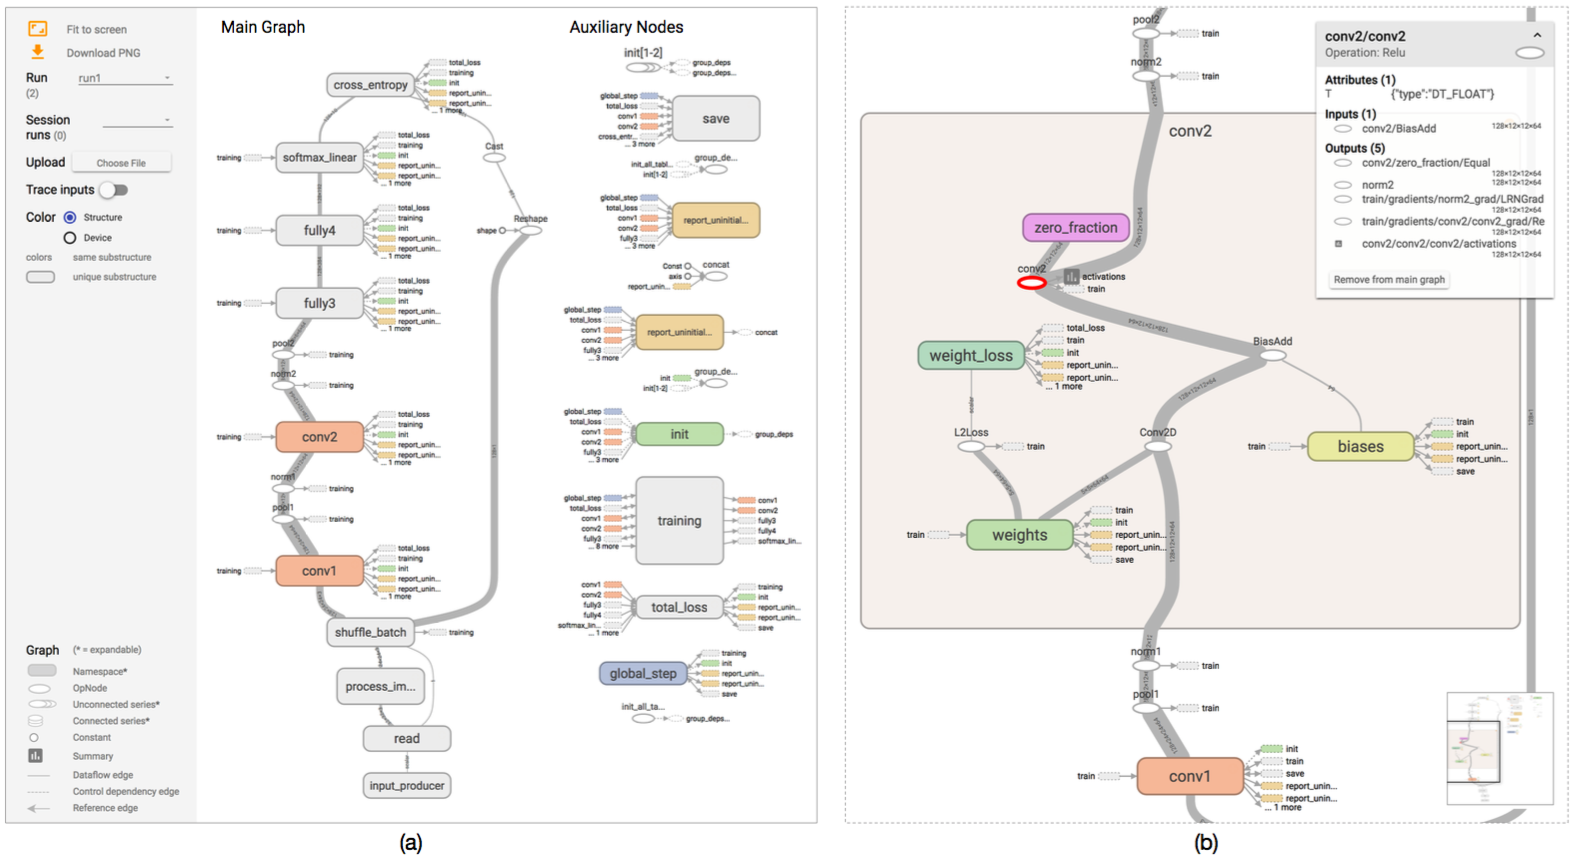
\includegraphics[width=1.0\textwidth]{figure/dataflow-graph}
    \caption{The TensorFlow Graph Visualizer shows a CNN image classifier \cite{wongsuphasawat2017dataflow}. (a) An overview displays a dataflow between groups of operations, with auxiliary nodes extracted to the side. (b) Expanding a group shows its nested structure.}
    \label{fig:dataflow-graph}
\end{figure}

\textbf{Code diagnosis.} Wongsuphasawat \etal \cite{wongsuphasawat2017dataflow} design and implemented a scalable graph layout for the data flow graph of any machine learning model and integrate the graph visualization in TensorFlow (see \autoref{fig:dataflow-graph}). The code defining the data flow graph can be automatically converted to a visualization, which helps developers validate the correctness of the code. A similar computation graph overview is proposed in the ActiVis, a visual exploration system for machine learning models developed by Kahng \etal \cite{kahng2017activis}.

\textbf{Training diagnosis.} There are also visual analytics systems developed to understand the training process of specific models. Unlike standard testing for software engineering, there is no accurate definition of the failure of a training. The failure of a training is a relative concepts. It is difficult to determine if a high loss is due to local optimum, the limitation of the model, or the quality of the dataset. Providing visual hints or indicator can help developers identify possible cause of failed training. The diagnosis of the training process is usually provided by sampling multiple snapshots during training. Liu \etal \cite{liu2017gan} develop the DGMTracker, which tracks the training process of the deep generative models (DGM) (\eg, generative adversarial model). They cache the training dynamics (\eg, activation changes) and visualize the training dynamics to help identify possible cause of a failed training. Pezzotti \etal \cite{pezzotti2017deep-eyes} proposed a progressive method that support the identification of layers that learn stable patterns and superfluous filters or layers. Visual analytics systems are also proved to be useful for tree boosting methods \cite{liu2017tree}. These visual analytics system are also model-specific and are difficult to generalize. There still needs further research in understanding the characteristics of the loss function to guide better the development of visualization techniques for training diagnosis.

\subsection{Assessment and Comparison} 

The purpose of evaluation is to determine if a trained classifier meets certain standards for deployment, and to select the best one among multiple classifiers. The evaluation is, to some extent, closely related to the training diagnostics. If a classifier fails the evaluation, then we will go back to adjust parameters for another training or refine its architecture. Visualization can also be used to assess and compare the performance of classifiers comprehensively (\eg, identify which classes the classifier is not good at). The visualization here also provide certain level of global explanations -- explaining a classifier using the statistics of its outputs of the test data. 

\begin{figure}[bt]
    \centering
    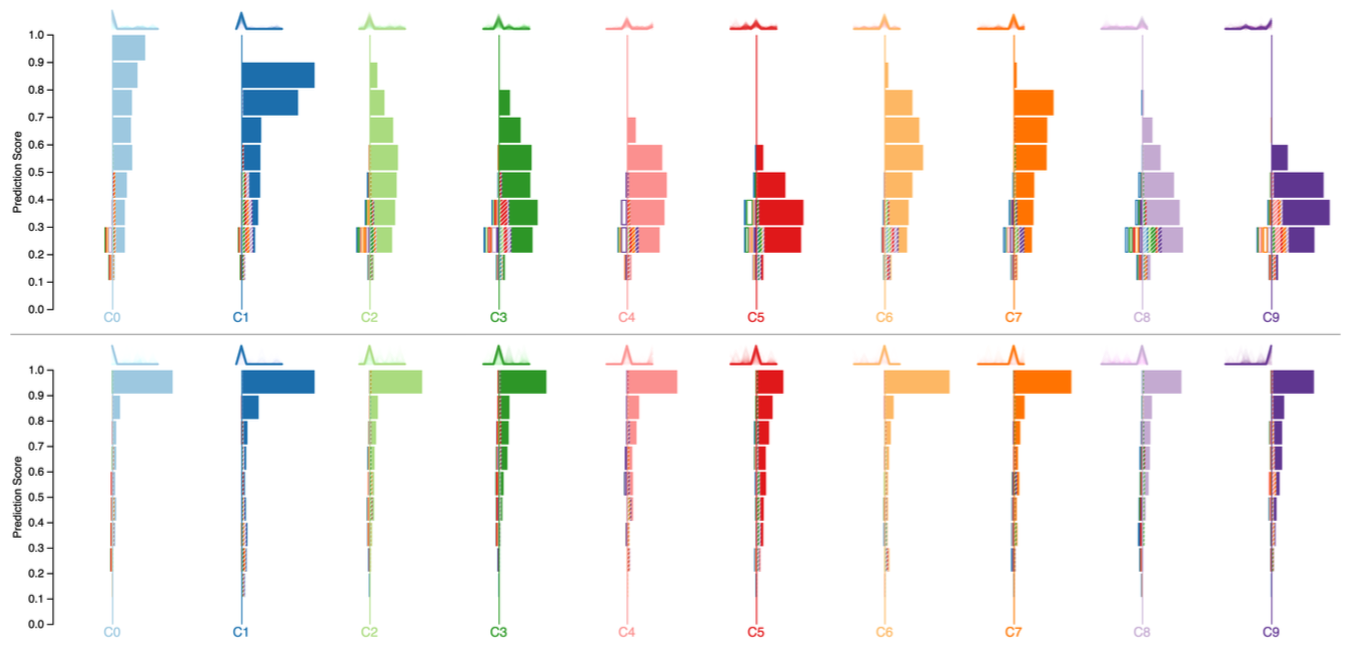
\includegraphics[width=1.0\textwidth]{figure/squares}
    \caption{Squares \cite{ren2017squares} displaying the performance of two classifier (top: random forest, bottom: SVM) trained on the MNIST dataset. They yield the same accuracy of 0.87 , but show vastly different score distributions.}
    \label{fig:squares}
\end{figure}

Amershi \etal \cite{amershi2015modeltracker} develop the ModelTracker to support the interactive performance analysis for binary classifier using stacked diagram. The ModelTracker combines the performance statistics and data inspection functions, which helps engineers evaluate the performance and identify problematic classifications at the same time.
Ren \etal extend it to the Squares \cite{ren2017squares}, which support the performance analysis for multi-class classifiers. As shown in \autoref{fig:squares}, the Squares is used to compare the performance of two classifiers, a random forest and an SVM, on the MNIST dataset. We can easily see that the SVM has much higher confidence than the random forest, though they have the same accuracy.
% \cite{muhlabacher2017treepod}

% There are plenty of opportunities to use visualization for evaluating and comparing classifiers. 

Currently, most evaluations only address accuracy and computation cost. As discussed in \autoref{sec-concepts}, we may need to meet other requirements such as fairness, robustness and explainability in certain applications. 
As discussed above, visualization can be used to enhance the explainability of a complex classifier. By explaining the reasoning of the classifier, we can identify possible discriminate classifications of the model. It is also possible to qualitatively evaluate the robustness of the classifier by verify if the classifier's reasoning matches that of a human or it is using unexpected reasoning. 

Except for the issues stated above, there are three general research issues for visualization in the model development stage. The first issue is the scalability of the visualization design. Many visualizations perform well in toy datasets such as MNIST. However, they will easily become overwhelming if the number of classes increases to a few hundreds. The second is the lack of consensus in the evaluation. The target of these visualization techniques is explaining and understanding, which is also subjective. It is difficult to design appropriate evaluation tasks for users to perform. The third is the need for a comprehensive toolkit that covers different procedures fluently. For example, TensorBoard\footnote{\url{https://github.com/tensorflow/tensorboard}} is a toolkit for visualizign and debugging machine learning models, which has been closely integrated in TensorFlow, but it is still at an early stage and has a limited set of functions.

\begin{figure}[bt]
    \centering
    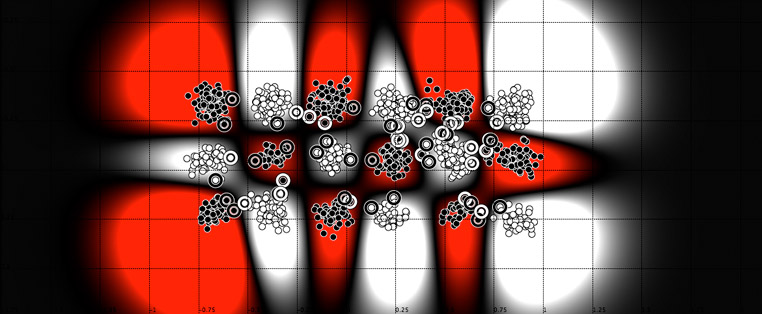
\includegraphics[width=1.0\textwidth]{figure/svm-rbf-points}
    \caption{A visualization from MLDemos, showing the decision space of a binary SVM classifier using RBF kernel. White and red denotes different classes, and black represents uncertainty.}
    \label{fig:mldemos}
\end{figure}

\subsection{Communication and Education}

Another related task, although not a necessary one in the model development stage, is the communicating and teaching of classification models. This task is related to the task of understanding. However, the focus of this task is not for a better understanding of the working mechanisms of a classifier, but for a better presentation of a classifier. 

% Visualization can directly help improve the explainability during the procedure of evaluation. There are other desirable properties except for a good accuracy, namely, fairness, robustness, and explainability. 

% Unquantifiable assessments, Fairness (e.g., discrimination), Vulnerability
With the growing complexity of model architectures, it often requires much effort to understand the composition and computation steps of a new classifier. It also requires a lot of work from the author to draw a diagram, which may neglect useful information for the readers. Netscope\footnote{\url{http://ethereon.github.io/netscope}} is a visualization tool that converts the code of a model written in Caffe\footnote{\url{http://caffe.berkeleyvision.org/}} to a node-link graph. Which helps quickly understand the topology of a model. However, the visualization will become too large if the model is complex (\eg, a CNN with a hundred layers), and it does not show extra information (\eg, optimizing method) about the model. TensorBoard utilizes the data flow graph visualization developed by Wongsuphasawat \cite{wongsuphasawat2017dataflow}, which is interactive and more scalable.

For new comers who want to learn, there will also be a large overhead to understand the computation of different components. Some visualizations have been developed to help people learn. Basilio Noris develops a visualization tool, MLDemos\footnote{\url{http://mldemos.epfl.ch/}} for understanding the behavior of various machine learning algorithms. As shown in \autoref{fig:mldemos}, MLDemos maps the output of a classifier using multiple colors back to the input space, and helps people learn the characteristics of different classifiers. Tensorflow Playground\footnote{\url{http://playground.tensorflow.org/}} is an interactive visualization, which helps people understand the behavior of a neural network, using similar techniques.


\section{Visualization for Operation}
The operation and management after deploying a classification system is an important stage of the whole life cycle, but  little attention has been paid to this stage. There are two common tasks that needs explainability: trust establishment and inspection.

\subsection{Trust Establishment}
The first challenge after the classifier has been deployed is how to establish users' trust in the machine.  Ribeiro \etal \cite{ribeiro2016kdd} have discussed the importance of a user's trust: if the user does not rust a model, he/she will not use it. If a user understand why the classifier predict class $A$ but not $B$, if he/she understand when the classifier performs well and when it is likely to fail, if he/she can figure out the possible reasons for a failure, he/she will trust the classifier. Thus, the foundation of trust is understanding, which can be achieved through explanation. Ribeiro \etal designed a inspiring solution for explanation, that is, locally approximate the complex classifier using an interpretable one, a linear classifier. Then the linear classifier is used to generate a local explanation (\eg, a list of words for a document classifier). Although this method introduces another classifier, whose error is not guaranteed, they showed that users indeed have more confident and trust in the classifier. Though explanation for trust establishment is promising, there are still unsolved issues. How to make sure the generated explanation is fidel to the model? How to evaluate whether the user has learned the correct message from the explanation? These should be addressed in future research.

\subsection{Monitoring}
After the end-users have established their trust in a classifier, they still needs a human-friendly interface to inspect or monitor the classifier. This need can be satisfied by providing faithful local explanations for specific predictions. The need for monitoring is not solely for preventing possible failure. For example, if we have developed a system for hospitals to detect early signs of lung cancer from CT scans, a good explanation not only helps the doctor correct possible false positives, but also provide the doctor extra information for deciding whether further examinations are needed. 



% \section{Evaluation}

% Review methods and standards of evaluating visualization.

% Address the problem of the lack of evaluation standards for visualization for explaianble classifiers.

% Proposed?

% 1. Fidelity. How visualization reflects the real model. (The relativeness and faithfulness of explanation)

% 2. Understandability. How easy the visualization is to be understood.

% \newpage


\chapter{Conclusion}\label{sec-conclusion}

Explainability is a critical but often-overlooked property for intelligent systems. In this survey, we review techniques that provide explainability to classifiers, with a special focus on visualization. We first discuss the concept and definition of explainability of a classifier. Two types of techniques that provide explainability to classifiers are summarized and discussed. Then based on the life cycle of intelligent systems, we discuss the role of visualization in different stages, and how visualization can be used to improve explainability.

The research in the explainability of classifiers is still a growing discipline. There is no consensus on the definition of explainability in the context of supervised learning. There is few rigorous evaluation methods of the explainability of a classifier or a explanation of a classifier. Early work treats the explainability as the ``simplicity'' and always focuses on balancing the trade-offs between performance and simplicity. Now there is a new trend of building an explanatory interface between human and the underlying model to enhance explainability while maintaining the performance. A few challenges and research issues are summarized as follows.

\textbf{Rigorous theory of explainability}. There are plenty of unsolved questions in the the seemly intuitive concept of explainability. How to rigorously define explainability in the context of machine learning or artificial intelligence? What is explanation? How to evaluate whether an explanation is good or not? How can we model the variation and uncertainty of human in the explanatory interface? Based on the theory of explainability, a further issue that needs to address is the \textbf{evaluation} of explainability and the quality of explanations. If a metric based evaluation is inapplicable, there still need guidelines for system designs. There is some work in cognitive science studying the function, structure of explanation, and the role that explanation plays in perception, cognition, and learning. It may be promising to learn from the theory from cognition science. Still, it requires the efforts from both cognitive science and computer science.

\textbf{Applications}. Theory comes from practice. Although there are toy examples, showing how explainability helps design better models, avoid possible bias, and enhance users' trust, we still lack knowledge on the design challenges of a explainable interface in real-world applications. Is it possible to let the machine explain its learned knowledge to a human? There are few successes or failures in real-world applications that we can learn from. Another neglected stakeholder is the end-users who actually use or are influenced by the technology developed based on AI. How do they value explainability during the use of an intelligent system? How can we use explanatory techniques to improve their using experience? The research at this end might be able to impact more people.

% \textbf{}


% \section{Other Applications}
% \subsection{Teaching and Communicating Models}
% \cite{harley2015isvc}
% Basilio Noris develop a visualization tool, MLDemos\footnote{\url{http://mldemos.epfl.ch/}}, for understanding how different algorithms and parameters influence the results in different machine learning problems. The tool project the decision space back to the input space,  how the output space of a classifier is 
% \cite{wongsuphasawat2017dataflow}
% Narrative, Interactive, etc. to explain your model to others.
% \subsection{Learn from the Model} 
% Knowledge Discovery; Learn lessons from what the model learned (Alpha Go)

%%%%%%%%%%%%%%%%%%%%%%%%%%%%%%%%%%%%%%%%%%%%%%%%%%%%%%%%%%%%%%%%%%%%%%%%%
%                                                                       %
%      9) BIBLIOGRAPHY                                                  %
%                                                                       %
% This example uses bibtex to generate the required Bibliography. Refer %
% to the % the file ustthesis_test.bib for the entries of the           %
% Bibliography. Note that only the cited entries are printed.           %
%                                                                       %
% If BibTeX is not used to typeset the bibliography, replace the        %
% following line with the \begin{thebibliography} and \end{bibliography}%
% commands (the "thebibliography" environment) to process the           %
% Bibliography.                                                         %
%                                                                       %
%%%%%%%%%%%%%%%%%%%%%%%%%%%%%%%%%%%%%%%%%%%%%%%%%%%%%%%%%%%%%%%%%%%%%%%%%

%%%%%%%%%%%%%%%%%%%%%%%%%%%%%%%%%%%%%%%%%%%%%%%%%%%%%%%%%%%%%%%%%%%%%%%%%
%                                                                       %
% The recommended bibliography style is the IEEE bibliography style.    %
% "ustbib" defines the IEEE bibliography standard with the added        %
% ability of sorting the items by name of author.                       %
%                                                                       %
% If you are not using BibTeX to process your Bibliography, comment out %
% the following line.                                                   %
%                                                                       %
%%%%%%%%%%%%%%%%%%%%%%%%%%%%%%%%%%%%%%%%%%%%%%%%%%%%%%%%%%%%%%%%%%%%%%%%%

\bibliographystyle{IEEETranS}

\bibliography{ref}
% Please run "bibtex ustthesis_test" before the bibliography can be
% included.

%%%%%%%%%%%%%%%%%%%%%%%%%%%%%%%%%%%%%%%%%%%%%%%%%%%%%%%%%%%%%%%%%%%%%%%%%
%                                                                       %
%     10) APPENDIX (If Any)                                              %
%                                                                       %
% \appendix command marks the beginning of the APPENDIX part of the     %
% Thesis. The usual \chapter command is used for the different chapters %
% of the Appendix.                                                      %
%                                                                       %
%%%%%%%%%%%%%%%%%%%%%%%%%%%%%%%%%%%%%%%%%%%%%%%%%%%%%%%%%%%%%%%%%%%%%%%%%


%%%%%%%%%%%%%%%%%%%%%%%%%%%%%%%%%%%%%%%%%%%%%%%%%%%%%%%%%%%%%%%%%%%%%%%%%
%                                                                       %
%     11) BIOGRAPHY (Optional)                                          %
%                                                                       %
% \biography and \endbiography are used to define the optional          %
% Biography of the author of the Thesis.                                %
%                                                                       %
%%%%%%%%%%%%%%%%%%%%%%%%%%%%%%%%%%%%%%%%%%%%%%%%%%%%%%%%%%%%%%%%%%%%%%%%%

% \biography
% The biography of the student is ALSO optional.
% \endbiography

\end{document}
